The DGMPM is now illustrated on numerical examples considering materials based on the Hencky hyperelastic-plastic potential presented in \cite{Laurent2009} and isotropic hardening. 
The values of the material parameters used are gathered in table \ref{tab:material}, the elastic behavior being given by Young's modulus $E$ and Poisson's ratio $\nu$. 
On the other hand, the plastic flow is governed by the yield stress in tension $\sigma^y$ and the hardening coefficient $H$ for a linear hardening, supplemented with the power law exponent $1/n$ for a non linear hardening.
\begin{table}[h!]
  \centering
    \begin{tabular}{l|l|lN}
    \hline
    $E=2\times 10^{11}\:Pa$ & $\sigma^y=4 \times 10^8 Pa$ & $n=4.37$&  \\ [3pt]
    $\nu=0.3$ & $H=10^{10} Pa$ & $\eta=\sigma^y \:\tau^{1/n} \: Pa.s$ & \\[3pt]
    $\rho = 7800 \: kg.m^{-3}$ & & &\\[3pt]
    \hline
  \end{tabular}

%%% Local Variables:
%%% mode: latex
%%% TeX-master: "../../mainManuscript"
%%% End:

  \caption{Material parameters.}
  \label{tab:material}
\end{table}

Moreover, the simulations carried out with the particle-based methods and presented in the section are based on the effective mass matrix defined in section \ref{sec:discretization}, which requires the setting of the parameter $\xi$.
Most of MPM computations that can be found in the literature are performed based on a lumped mass matrix \cite{Book_MPM,MPM_PIC_FLIP,MPM_cutting,BC_MPM}, in such a way that no value of the parameter $\xi$ is recommended.
In addition, since so stability analysis of the scheme exists, the same goes for the critical Courant number which is usually set to CFL$=0.5$ or CFL=$0.7$ though it is not proofed mathematically.
Contrariwise, the stability analysis of the DGMPM based on a lumped mass matrix enables the computation of the optimal CFL number for a given distribution of material points for one-dimensional problems \cite{DGMPM} and two-dimensional ones \cite{DGMPM_stab}.
It furthermore appears that the value of the critical Courant number also corresponds to a good choice for the parameter $\xi$ in order to balance the numerical diffusion and the stability.
As a result, the CFL values given in the following also go for $\xi$ in DGMPM computations.
On the other hand, the Courant number used in MPM simulations is set to CFL$=0.5$ while the parameter $\xi$ is identical to this used in the DGMPM for comparison purposes. 

\begin{remark}
  The use of the effective mass matrix within the DGMPM must have an influence on the consistency of the method.
  Nevertheless, since the DGMPM using a lumped mass matrix is first-order accurate \cite{Thesis}, the implementation used here can only exhibit a higher or equivalent convergence rate.
\end{remark}

\subsection{Plane wave problem}
\label{sec:plane-wave-problem}
Let's first look at the response of an infinite medium in directions $\vect{e}_2$ and $\vect{e}_3$ and of length $l=1\:m$ in direction $\vect{e}_1$, to Riemann-type initial conditions defined on the velocity: $v_1=v_d>0$ for $X\in[0,l/2[$ and $v_1=-v_d$ for $X \in ]l/2,l]$.
Initially, the solid is in a free stress state and the velocity is set so that plastic flow occurs:
\begin{equation*}
  v_d=\beta \frac{Y_H}{\rho c_L}
\end{equation*}
where $\beta$ is a loading parameter, $Y_H=(\lambda+2\mu)\sigma^y/2\mu$ denotes the Hugoniot elastic limit, $c_L=\sqrt{(\lambda+2\mu)/\rho}$ is the elastic pressure wave speed, and $(\lambda,\mu)$ are Lam\'e's constants.
Both ends of the medium are traction free.
The initial setting is assumed to give rise to a plane wave, namely:
\begin{align*}
  & \tens{F}= F \vect{e}_1 \otimes\vect{e}_1 + \vect{e}_2 \otimes\vect{e}_2 + \vect{e}_3 \otimes\vect{e}_3\\
  & \tens{\Pi}=\Pi_L \vect{e}_1 \otimes \vect{e}_1 + \Pi_T \(\vect{e}_2 \otimes \vect{e}_2+\vect{e}_3 \otimes \vect{e}_3\) 
\end{align*}
Comparisons between FEM, MPM and DGMPM solutions are proposed on the longitudinal components of the PK1 stress and the Green-Lagrange plastic strain $\tens{E}^p=\frac{1}{2}\({\tens{F}^p}^T\tens{F}^p - \tens{I}\)$.
Linear elements and a lumped mass matrix are used within FEM with no artificial viscosity added, and the regular mesh is built so that Gauss' points are consistent with the particles, the solid being discretized with $100$ finite elements and particles.
The space discretization used within the MPM and the DGMPM can be based on either one single particle centered in every cell, or two particles in each element that are placed symmetrically with respect to the center.
The aforementioned discretizations are respectively referred to as 1ppc and 2ppc, ppc standing for point per cell.
It is in addition noteworthy that all numerical methods are based on a total Lagrangian formulation and make use of the same variational constitutive update.

\begin{figure}[h!]
  \centering
  {\phantomsubcaption{\label{subfig:he_planeWave1}}}
  {\phantomsubcaption{\label{subfig:he_planeWave2}}}
  {\phantomsubcaption{\label{subfig:he_planeWave3}}}
  \begin{tikzpicture}[spy using outlines={rectangle, magnification=3, size=1.cm, connect spies},scale=.8]
  \begin{groupplot}[group style={group size=3 by 2,ylabels at=edge left, yticklabels at=edge left,horizontal sep=2.ex,vertical sep=4ex,xticklabels at=edge bottom,xlabels at=edge bottom},ymajorgrids=true,xmajorgrids=true,enlargelimits=0,xmin=0.5,xmax=1.,xlabel=$x (m)$,axis on top,scale only axis,width=0.33\linewidth,height=0.25\linewidth]

    % ============================== Stress Line
    % t1 % t= 6.84e-5
    \nextgroupplot[title={(a) $t = 6.84\times 10^{-5} $ s.},ylabel=$\Pi_L \: (Pa)$,ymin=-8.5e8,ymax=8.e8]
    \addplot[Red,densely dashed,thick] table[x=x,y=Pi] {pgfFigures/HEP_planeWave/mpm0.pgf};
    \addplot[Green,densely dotted,very thick] table[x=x,y=Pi] {pgfFigures/HEP_planeWave/mpm_2ppc0.pgf};
    \addplot[Blue,mark=asterisk,thick,mark repeat=2,mark size=3pt] table[x=x,y=Pi] {pgfFigures/HEP_planeWave/dgmpm0.pgf};
    %\addplot[Purple,mark=x,thick,mark repeat=2,mark size=3pt] table[x=x,y=Pi] {pgfFigures/HEP_planeWave/dgmpm_2ppc0.pgf};
    \addplot[Purple,mark=x,thick,mark repeat=2,mark size=3pt] table[x=x,y=Pi] {pgfFigures/HEP_planeWave/dgmpm_2ppc_effective0.pgf};
    \addplot[Orange,mark=*,thick,mark repeat=2,mark size=2pt] table[x=x,y=Pi] {pgfFigures/HEP_planeWave/fem0.pgf};
    \addplot[black] table[x=x,y=Pi] {pgfFigures/HEP_planeWave/exact0.pgf};

    \begin{scope}
      \spy[black,size=1.5cm] on (2.8,0.25) in node [fill=none] at (2.725,3.);
    \end{scope}

    % t2 % t= 1.37e-4
    \nextgroupplot[title={(b) $t=1.37\times 10^{-4}$ s.},ymin=-8.5e8,ymax=8.e8]
    \addplot[Red,densely dashed,thick] table[x=x,y=Pi] {pgfFigures/HEP_planeWave/mpm1.pgf};
    \addplot[Green,densely dotted,very thick] table[x=x,y=Pi] {pgfFigures/HEP_planeWave/mpm_2ppc1.pgf};
    \addplot[Blue,mark=asterisk,thick,mark repeat=2,mark size=3pt] table[x=x,y=Pi] {pgfFigures/HEP_planeWave/dgmpm1.pgf};
    \addplot[Purple,mark=x,thick,mark repeat=2,mark size=3pt] table[x=x,y=Pi] {pgfFigures/HEP_planeWave/dgmpm_2ppc1.pgf};
    %\addplot[Yellow,mark=+,thick,mark repeat=2,mark size=3pt] table[x=x,y=Pi] {pgfFigures/HEP_planeWave/dgmpm_2ppc_effective1.pgf};
    \addplot[Orange,mark=*,thick,mark repeat=2,mark size=2pt] table[x=x,y=Pi] {pgfFigures/HEP_planeWave/fem1.pgf};
    \addplot[black] table[x=x,y=Pi] {pgfFigures/HEP_planeWave/exact1.pgf};


    % \begin{scope}
    %   \spy[black,size=1.5cm] on (7.2,1.5) in node [fill=none] at (6.75,3.);
    % \end{scope}

    
    % t3 % t= 2.05e-4
    \nextgroupplot[title={(c) $t=2.05\times 10^{-4}$ s.},ymin=-8.5e8,ymax=8.e8]
    \addplot[Red,densely dashed,thick] table[x=x,y=Pi] {pgfFigures/HEP_planeWave/mpm2.pgf};
    \addplot[Green,densely dotted,very thick] table[x=x,y=Pi] {pgfFigures/HEP_planeWave/mpm_2ppc2.pgf};
    \addplot[Blue,mark=asterisk,thick,mark repeat=2,mark size=3pt] table[x=x,y=Pi] {pgfFigures/HEP_planeWave/dgmpm2.pgf};
    \addplot[Purple,mark=x,thick,mark repeat=2,mark size=3pt] table[x=x,y=Pi] {pgfFigures/HEP_planeWave/dgmpm_2ppc2.pgf};
    %\addplot[Yellow,mark=+,thick,mark repeat=2,mark size=3pt] table[x=x,y=Pi] {pgfFigures/HEP_planeWave/dgmpm_2ppc_effective2.pgf};
    \addplot[Orange,mark=*,thick,mark repeat=2,mark size=2pt] table[x=x,y=Pi] {pgfFigures/HEP_planeWave/fem2.pgf};
    \addplot[black] table[x=x,y=Pi] {pgfFigures/HEP_planeWave/exact2.pgf};
    
    % \begin{scope}
    %   \spy[black,size=1.5cm] on (9.65+2.,3.5) in node [fill=none] at (11+3.2,1.25);
    % \end{scope}

    % ============================== Plastic strain Line
    % t1
    \nextgroupplot[ylabel=$E^p_{11}$,ymin=-1.12e-3,ymax=2.e-4]
    \addplot[Red,densely dashed,thick] table[x=x,y=epls] {pgfFigures/HEP_planeWave/mpm0.pgf};
    \addplot[Green,densely dotted,very thick] table[x=x,y=epls] {pgfFigures/HEP_planeWave/mpm_2ppc0.pgf};
    \addplot[Blue,mark=asterisk,thick,mark repeat=2,mark size=3pt] table[x=x,y=epls] {pgfFigures/HEP_planeWave/dgmpm0.pgf};
    \addplot[Purple,mark=x,thick,mark repeat=2,mark size=3pt] table[x=x,y=epls] {pgfFigures/HEP_planeWave/dgmpm_2ppc0.pgf};
    %\addplot[Yellow,mark=+,thick,mark repeat=2,mark size=3pt] table[x=x,y=epls] {pgfFigures/HEP_planeWave/dgmpm_2ppc_effective0.pgf};
    \addplot[Orange,mark=*,thick,mark repeat=2,mark size=2pt] table[x=x,y=epls] {pgfFigures/HEP_planeWave/fem0.pgf};
    \addplot[black] table[x=x,y=epls] {pgfFigures/HEP_planeWave/exact0.pgf};
    
    % t2
    \nextgroupplot[legend style={at={($(0.9,-0.45)+(2.1cm,0.65cm)$)},legend columns=3},ymin=-1.12e-3,ymax=2.e-4]
    \addplot[Red,densely dashed,thick] table[x=x,y=epls] {pgfFigures/HEP_planeWave/mpm1.pgf};
    \addplot[Green,densely dotted,very thick] table[x=x,y=epls] {pgfFigures/HEP_planeWave/mpm_2ppc1.pgf};
    \addplot[Blue,mark=asterisk,thick,mark repeat=2,mark size=3pt] table[x=x,y=epls] {pgfFigures/HEP_planeWave/dgmpm1.pgf};
    \addplot[Purple,mark=x,thick,mark repeat=2,mark size=3pt] table[x=x,y=epls] {pgfFigures/HEP_planeWave/dgmpm_2ppc1.pgf};
    %\addplot[Yellow,mark=+,thick,mark repeat=2,mark size=3pt] table[x=x,y=epls] {pgfFigures/HEP_planeWave/dgmpm_2ppc_effective1.pgf};
    
    \addplot[Orange,mark=*,thick,mark repeat=2,mark size=2pt] table[x=x,y=epls] {pgfFigures/HEP_planeWave/fem1.pgf};
    \addplot[black] table[x=x,y=epls] {pgfFigures/HEP_planeWave/exact1.pgf};
    
    \addlegendentry{mpm (1ppc)}
    \addlegendentry{mpm (2ppc)}
    \addlegendentry{dgmpm (1ppc)}
    \addlegendentry{dgmpm (2ppc)}
    %\addlegendentry{dgmpm (2ppc) -- effective}
    \addlegendentry{fem}
    \addlegendentry{exact}
    % t3
    \nextgroupplot[,ymin=-1.12e-3,ymax=2.e-4]
    \addplot[Red,densely dashed,thick] table[x=x,y=epls] {pgfFigures/HEP_planeWave/mpm2.pgf};
    \addplot[Green,densely dotted,very thick] table[x=x,y=epls] {pgfFigures/HEP_planeWave/mpm_2ppc2.pgf};
    \addplot[Blue,mark=asterisk,thick,mark repeat=2,mark size=3pt] table[x=x,y=epls] {pgfFigures/HEP_planeWave/dgmpm2.pgf};
    \addplot[Purple,mark=x,thick,mark repeat=2,mark size=3pt] table[x=x,y=epls] {pgfFigures/HEP_planeWave/dgmpm_2ppc2.pgf};
    %\addplot[Yellow,mark=+,thick,mark repeat=2,mark size=3pt] table[x=x,y=epls] {pgfFigures/HEP_planeWave/dgmpm_2ppc_effective2.pgf};
    
    \addplot[Orange,mark=*,thick,mark repeat=2,mark size=2pt] table[x=x,y=epls] {pgfFigures/HEP_planeWave/fem2.pgf};
    \addplot[black] table[x=x,y=epls] {pgfFigures/HEP_planeWave/exact2.pgf};

  \end{groupplot}
\end{tikzpicture}



%%% Local Variables:
%%% mode: latex
%%% TeX-master: "../manuscript"
%%% End:

  \caption{Longitudinal components of PK1 stress and plastic Green-Lagrange strain tensors along a one-dimensional hyperelastic-plastic domain subject to Riemann-type initial conditions on the velocity at different times. Comparison between FEM (CFL=1), MPM (CFL=0.5), DGMPM using one particle per cell (CFL=1) or two particles per cell (CFL=0.5), and the exact solution of the small strain problem.}
  \label{fig:hep_planeWave}
\end{figure}
The parameter $\beta$ is first set to $1.2$ so that the problem falls within the linearized geometrical limit $\norm{\tens{F}} \ll 1$.
Then, considering linear isotropic hardening, the computed hyperelastic-plastic solution should tend to the elastoplastic one derived in \cite{Thomas_EP}.
The latter consists of two elastic compression waves propagating left-ward and right-ward, each followed by one plastic discontinuity.
The incident elastic disturbances then reflect as unloading waves on both free boundaries and then interact at the center of the medium, which leads to tensile plastic reloading.
In figure \ref{fig:hep_planeWave}, the numerical solutions provided by the DGMPM, the MPM and the FEM are compared to the exact solution of the small strain problem in the right half of the domain, given the symmetry of the problem.
\begin{figure}[h!]
  \centering
  {\phantomsubcaption{\label{subfig:he_planeWave_high_a}}}
  {\phantomsubcaption{\label{subfig:he_planeWave_high_b}}}
  {\phantomsubcaption{\label{subfig:he_planeWave_high_c}}}
  {\phantomsubcaption{\label{subfig:he_planeWave_high_d}}}
  {\phantomsubcaption{\label{subfig:he_planeWave_high_e}}}
  {\phantomsubcaption{\label{subfig:he_planeWave_high_f}}}
  {\phantomsubcaption{\label{subfig:he_planeWave_high_g}}}
  {\phantomsubcaption{\label{subfig:he_planeWave_high_h}}}
  {\phantomsubcaption{\label{subfig:he_planeWave_high_i}}}
  \begin{tikzpicture}[spy using outlines={rectangle, magnification=4, size=.5cm, connect spies},scale=.8]
  \begin{groupplot}[group style={group size=3 by 2,ylabels at=edge left, yticklabels at=edge left,horizontal sep=4.ex,vertical sep=4ex,xticklabels at=edge bottom,xlabels at=edge bottom},ymajorgrids=true,xmajorgrids=true,enlargelimits=0,xmin=0.5,xmax=1.,xlabel=$x (m)$,axis on top,scale only axis,width=0.33\linewidth,height=0.17\linewidth]

    % ============================== Stress Line
    % t1 % t= 6.84e-5
    \nextgroupplot[title={(a) $t = 7.92\times 10^{-5} $ s.},ylabel=$\Pi_L \: (Pa)$
    ,ymin=-3.e9,ymax=0.
    ]
    \addplot[Red,densely dashed,thick] table[x=x,y=Pi] {pgfFigures/HEP_planeWave/mpm_high_0.pgf};
    \addplot[Blue,mark=asterisk,thick,mark repeat=4,mark size=2pt] table[x=x,y=Pi] {pgfFigures/HEP_planeWave/dgmpm_high_0.pgf};
    \addplot[Purple,mark=x,thick,mark repeat=4,mark size=2pt] table[x=x,y=Pi] {pgfFigures/HEP_planeWave/dgmpm_2ppc_high_0.pgf};
    \addplot[black,thick] table[x=x,y=Pi] {pgfFigures/HEP_planeWave/fem_high_0.pgf};

    
    % t2 % t= 1.37e-4
    \nextgroupplot[title={(b) $t=8.93\times 10^{-5}$ s.}
    ,ymin=-3e9,ymax=0.
    ]
    \addplot[Red,densely dashed,thick] table[x=x,y=Pi] {pgfFigures/HEP_planeWave/mpm_high_1.pgf};
    \addplot[Blue,mark=asterisk,thick,mark repeat=4,mark size=2pt] table[x=x,y=Pi] {pgfFigures/HEP_planeWave/dgmpm_high_1.pgf};
    \addplot[Purple,mark=x,thick,mark repeat=4,mark size=2pt] table[x=x,y=Pi] {pgfFigures/HEP_planeWave/dgmpm_2ppc_high_1.pgf};
    \addplot[black,thick] table[x=x,y=Pi] {pgfFigures/HEP_planeWave/fem_high_1.pgf};

    % t3 % t= 2.05e-4
    \nextgroupplot[title={(c) $t=1.01\times 10^{-4}$ s.}
    ,ymin=-3e9,ymax=0.
    ]
    \addplot[Red,densely dashed,thick] table[x=x,y=Pi] {pgfFigures/HEP_planeWave/mpm_high_2.pgf};
    \addplot[Blue,mark=asterisk,thick,mark repeat=4,mark size=2pt] table[x=x,y=Pi] {pgfFigures/HEP_planeWave/dgmpm_high_2.pgf};
    \addplot[Purple,mark=x,thick,mark repeat=4,mark size=2pt] table[x=x,y=Pi] {pgfFigures/HEP_planeWave/dgmpm_2ppc_high_2.pgf};
    \addplot[black,thick] table[x=x,y=Pi] {pgfFigures/HEP_planeWave/fem_high_2.pgf};
    \begin{scope}
      \spy[black,size=1.5cm] on (13.8,1.75) in node [fill=none] at (13.2,1.75);
    \end{scope}

    % ============================== Plastic strain Line
    % t1
    \nextgroupplot[ylabel=$E^p_{11}$,ymin=-.9e-2,ymax=0.]
    \addplot[Red,densely dashed,thick] table[x=x,y=epls] {pgfFigures/HEP_planeWave/mpm_high_0.pgf};
    \addplot[Blue,mark=asterisk,thick,mark repeat=4,mark size=2pt] table[x=x,y=epls] {pgfFigures/HEP_planeWave/dgmpm_high_0.pgf};
    \addplot[Purple,mark=x,thick,mark repeat=4,mark size=2pt] table[x=x,y=epls] {pgfFigures/HEP_planeWave/dgmpm_2ppc_high_0.pgf};
    \addplot[black,thick] table[x=x,y=epls] {pgfFigures/HEP_planeWave/fem_high_0.pgf};
    
    % t2
    \nextgroupplot[legend style={at={($(0.9,-0.45)+(2.25cm,.25cm)$)},legend columns=5},ymin=-.9e-2,ymax=0.]
    \addplot[Red,densely dashed,thick] table[x=x,y=epls] {pgfFigures/HEP_planeWave/mpm_high_1.pgf};
    \addplot[Blue,mark=asterisk,thick,mark repeat=4,mark size=2pt] table[x=x,y=epls] {pgfFigures/HEP_planeWave/dgmpm_high_1.pgf};
    \addplot[Purple,mark=x,thick,mark repeat=4,mark size=2pt] table[x=x,y=epls] {pgfFigures/HEP_planeWave/dgmpm_2ppc_high_1.pgf};
    
    \addplot[black,thick] table[x=x,y=epls] {pgfFigures/HEP_planeWave/fem_high_1.pgf};
    
    % \addlegendentry{mpm}
    % \addlegendentry{dgmpm (1ppc)}
    % \addlegendentry{dgmpm (2ppc)}
    % \addlegendentry{fem}
    % t3
    \nextgroupplot[,ymin=-.9e-2,ymax=0.] % 3.e-3 if exact solution is depicted
    \addplot[Red,densely dashed,thick] table[x=x,y=epls] {pgfFigures/HEP_planeWave/mpm_high_2.pgf};
    \addplot[Blue,mark=asterisk,thick,mark repeat=4,mark size=2pt] table[x=x,y=epls] {pgfFigures/HEP_planeWave/dgmpm_high_2.pgf};
    \addplot[Purple,mark=x,thick,mark repeat=4,mark size=2pt] table[x=x,y=epls] {pgfFigures/HEP_planeWave/dgmpm_2ppc_high_2.pgf};
    
    \addplot[black,thick] table[x=x,y=epls] {pgfFigures/HEP_planeWave/fem_high_2.pgf};

    % \begin{scope}
    %   \spy[black,size=2.cm] on (13.2,-1.95) in node [fill=none] at (14.25,-2.);
    % \end{scope}

  \end{groupplot}

  % %% plastic wave in figure 2
  % \draw[very thick,Green,->] (8.,2.25) -- (8.7,2.25);
  % %% elastic wave in figure 2
  % \draw[very thick,Green,->] (9.5,3.5) -- (8.8,3.5);
  % %% plastic wave in figure 3
  % \draw[very thick,Green,->] (14.5,-2.) -- (15.5,-2.);

\end{tikzpicture}



%%% Local Variables:
%%% mode: latex
%%% TeX-master: "../manuscript"
%%% End:

  \begin{tikzpicture}[spy using outlines={rectangle, magnification=4, size=.5cm, connect spies},scale=.8]
  \begin{groupplot}[group style={group size=3 by 2,ylabels at=edge left, yticklabels at=edge left,horizontal sep=4.ex,vertical sep=4ex,xticklabels at=edge bottom,xlabels at=edge bottom},ymajorgrids=true,xmajorgrids=true,enlargelimits=0,xmin=0.5,xmax=1.,xlabel=$x (m)$,axis on top,scale only axis,width=0.33\linewidth,height=0.17\linewidth]

    % ============================== Stress Line
    % t1 % t= 6.84e-5
    \nextgroupplot[title={(d) $t = 1.50\times 10^{-4} $ s.},ylabel=$\Pi_L \: (Pa)$
    ,ymin=-3.e9,ymax=0.
    ]
    \addplot[Red,densely dashed,thick] table[x=x,y=Pi] {pgfFigures/HEP_planeWave/mpm_high_3.pgf};
    \addplot[Green,densely dotted,very thick] table[x=x,y=Pi] {pgfFigures/HEP_planeWave/mpm_2ppc_high_3.pgf};
\addplot[Blue,mark=asterisk,thick,mark repeat=4,mark size=2pt] table[x=x,y=Pi] {pgfFigures/HEP_planeWave/dgmpm_high_3.pgf};
    \addplot[Purple,mark=x,thick,mark repeat=4,mark size=2pt] table[x=x,y=Pi] {pgfFigures/HEP_planeWave/dgmpm_2ppc_high_3.pgf};
    \addplot[black,thick] table[x=x,y=Pi] {pgfFigures/HEP_planeWave/fem_high_3.pgf};


    % t2 % t= 1.37e-4
    \nextgroupplot[title={(e) $t=1.73\times 10^{-4}$ s.}
    ,ymin=-3e9,ymax=0.
    ]
    \addplot[Red,densely dashed,thick] table[x=x,y=Pi] {pgfFigures/HEP_planeWave/mpm_high_4.pgf};
    \addplot[Green,densely dotted,very thick] table[x=x,y=Pi] {pgfFigures/HEP_planeWave/mpm_2ppc_high_4.pgf};
    \addplot[Blue,mark=asterisk,thick,mark repeat=4,mark size=2pt] table[x=x,y=Pi] {pgfFigures/HEP_planeWave/dgmpm_high_4.pgf};
    \addplot[Purple,mark=x,thick,mark repeat=4,mark size=2pt] table[x=x,y=Pi] {pgfFigures/HEP_planeWave/dgmpm_2ppc_high_4.pgf};
    \addplot[black,thick] table[x=x,y=Pi] {pgfFigures/HEP_planeWave/fem_high_4.pgf};
    %\addplot[black] table[x=x,y=Pi] {pgfFigures/HEP_planeWave/exact_high_4.pgf};
    
    % t3 % t= 2.05e-4
    \nextgroupplot[title={(f) $t=1.84\times 10^{-4}$ s.}
    ,ymin=-3e9,ymax=0.
    ]
    \addplot[Red,densely dashed,thick] table[x=x,y=Pi] {pgfFigures/HEP_planeWave/mpm_high_5.pgf};
    \addplot[Green,densely dotted,very thick] table[x=x,y=Pi] {pgfFigures/HEP_planeWave/mpm_2ppc_high_5.pgf};
    \addplot[Blue,mark=asterisk,thick,mark repeat=4,mark size=2pt] table[x=x,y=Pi] {pgfFigures/HEP_planeWave/dgmpm_high_5.pgf};
    \addplot[Purple,mark=x,thick,mark repeat=4,mark size=2pt] table[x=x,y=Pi] {pgfFigures/HEP_planeWave/dgmpm_2ppc_high_5.pgf};
    \addplot[black,thick] table[x=x,y=Pi] {pgfFigures/HEP_planeWave/fem_high_5.pgf};
    %\addplot[black] table[x=x,y=Pi] {pgfFigures/HEP_planeWave/exact_high_5.pgf};

    % ============================== Plastic strain Line
    % t1
    \nextgroupplot[ylabel=$E^p_{11}$,ymin=-0.9e-2,ymax=0.]
    \addplot[Red,densely dashed,thick] table[x=x,y=epls] {pgfFigures/HEP_planeWave/mpm_high_3.pgf};
    \addplot[Green,densely dotted,very thick] table[x=x,y=epls] {pgfFigures/HEP_planeWave/mpm_2ppc_high_3.pgf};
    \addplot[Blue,mark=asterisk,thick,mark repeat=4,mark size=2pt] table[x=x,y=epls] {pgfFigures/HEP_planeWave/dgmpm_high_3.pgf};
    \addplot[Purple,mark=x,thick,mark repeat=4,mark size=2pt] table[x=x,y=epls] {pgfFigures/HEP_planeWave/dgmpm_2ppc_high_3.pgf};
    \addplot[black,thick] table[x=x,y=epls] {pgfFigures/HEP_planeWave/fem_high_3.pgf};
    %\addplot[black] table[x=x,y=epls] {pgfFigures/HEP_planeWave/exact_high_3.pgf};
    
    % t2
    \nextgroupplot[legend style={at={($(0.9,-0.45)+(2.25cm,0.25cm)$)},legend columns=5},ymin=-0.9e-2,ymax=0.]
    \addplot[Red,densely dashed,thick] table[x=x,y=epls] {pgfFigures/HEP_planeWave/mpm_high_4.pgf};
    \addplot[Green,densely dotted,very thick] table[x=x,y=epls] {pgfFigures/HEP_planeWave/mpm_2ppc_high_4.pgf};
    \addplot[Blue,mark=asterisk,thick,mark repeat=4,mark size=2pt] table[x=x,y=epls] {pgfFigures/HEP_planeWave/dgmpm_high_4.pgf};
    \addplot[Purple,mark=x,thick,mark repeat=4,mark size=2pt] table[x=x,y=epls] {pgfFigures/HEP_planeWave/dgmpm_2ppc_high_4.pgf};
    
    \addplot[black,thick] table[x=x,y=epls] {pgfFigures/HEP_planeWave/fem_high_4.pgf};
    \begin{scope}
      \spy[black,size=1.cm] on (4.22,-.625) in node [fill=none] at (4.2,-2.7);
    \end{scope}
    
    % t3
    \nextgroupplot[,ymin=-0.9e-2,ymax=0.] % 3.e-3 if exact solution is depicted
    \addplot[Red,densely dashed,thick] table[x=x,y=epls] {pgfFigures/HEP_planeWave/mpm_high_5.pgf};
    \addplot[Green,densely dotted,very thick] table[x=x,y=epls] {pgfFigures/HEP_planeWave/mpm_2ppc_high_5.pgf};
    \addplot[Blue,mark=asterisk,thick,mark repeat=4,mark size=2pt] table[x=x,y=epls] {pgfFigures/HEP_planeWave/dgmpm_high_5.pgf};
    \addplot[Purple,mark=x,thick,mark repeat=4,mark size=2pt] table[x=x,y=epls] {pgfFigures/HEP_planeWave/dgmpm_2ppc_high_5.pgf};
    
    \addplot[black,thick] table[x=x,y=epls] {pgfFigures/HEP_planeWave/fem_high_5.pgf};
    % \begin{scope}
    %   \spy[black,size=1.cm] on (13.92,-.625) in node [fill=none] at (15.2,-2.7);
    % \end{scope}

  \end{groupplot}

  % elastic and plastic waves in the center
  % \draw[very thick,Green,->] (3.25,1.) -- (4.25,1);
\end{tikzpicture}



%%% Local Variables:
%%% mode: latex
%%% TeX-master: "../manuscript"
%%% End:

  \begin{tikzpicture}[spy using outlines={rectangle, magnification=3, size=1.cm, connect spies},scale=.8]
  \begin{groupplot}[group style={group size=3 by 2,ylabels at=edge left, yticklabels at=edge left,horizontal sep=4.ex,vertical sep=4ex,xticklabels at=edge bottom,xlabels at=edge bottom},ymajorgrids=true,xmajorgrids=true,enlargelimits=0,xmin=0.5,xmax=1.,xlabel=$x (m)$,axis on top,scale only axis,width=0.33\linewidth,height=0.17\linewidth]

    % ============================== Stress Line
    % t1 % t= 6.84e-5
    \nextgroupplot[title={(g) $t = 1.95\times 10^{-5} $ s.},ylabel=$\Pi_L \: (Pa)$
    ,ymin=-3.e8,ymax=2.25e9
    ]
    \addplot[Red,densely dashed,thick] table[x=x,y=Pi] {pgfFigures/HEP_planeWave/mpm_high_6.pgf};
    \addplot[Blue,mark=asterisk,thick,mark repeat=4,mark size=2pt] table[x=x,y=Pi] {pgfFigures/HEP_planeWave/dgmpm_high_6.pgf};
    \addplot[Purple,mark=x,thick,mark repeat=4,mark size=2pt] table[x=x,y=Pi] {pgfFigures/HEP_planeWave/dgmpm_2ppc_high_6.pgf};
    %\addplot[Orange,mark=*,thick,mark repeat=4,mark size=1pt] table[x=x,y=Pi] {pgfFigures/HEP_planeWave/fem_high_6.pgf};
    \addplot[black,thick] table[x=x,y=Pi] {pgfFigures/HEP_planeWave/fem_high_6.pgf};
    
    % t2 % t= 1.37e-4
    \nextgroupplot[title={(h) $t=2.06\times 10^{-4}$ s.}
    ,ymin=-3.e8,ymax=2.25e9
    ]
    \addplot[Red,densely dashed,thick] table[x=x,y=Pi] {pgfFigures/HEP_planeWave/mpm_high_7.pgf};
    \addplot[Blue,mark=asterisk,thick,mark repeat=4,mark size=2pt] table[x=x,y=Pi] {pgfFigures/HEP_planeWave/dgmpm_high_7.pgf};
    \addplot[Purple,mark=x,thick,mark repeat=4,mark size=2pt] table[x=x,y=Pi] {pgfFigures/HEP_planeWave/dgmpm_2ppc_high_7.pgf};
    %\addplot[Orange,mark=*,thick,mark repeat=4,mark size=1pt] table[x=x,y=Pi] {pgfFigures/HEP_planeWave/fem_high_7.pgf};
    \addplot[black,thick] table[x=x,y=Pi] {pgfFigures/HEP_planeWave/fem_high_7.pgf};
    
    % t3 % t= 2.05e-4
    \nextgroupplot[title={(i) $t=2.54\times 10^{-4}$ s.}
    ,ymin=-3.e8,ymax=2.25e9
    ]
    \addplot[Red,densely dashed,thick] table[x=x,y=Pi] {pgfFigures/HEP_planeWave/mpm_high_8.pgf};
    \addplot[Blue,mark=asterisk,thick,mark repeat=4,mark size=2pt] table[x=x,y=Pi] {pgfFigures/HEP_planeWave/dgmpm_high_8.pgf};
    \addplot[Purple,mark=x,thick,mark repeat=4,mark size=2pt] table[x=x,y=Pi] {pgfFigures/HEP_planeWave/dgmpm_2ppc_high_8.pgf};
    %\addplot[Orange,mark=*,thick,mark repeat=4,mark size=1pt] table[x=x,y=Pi] {pgfFigures/HEP_planeWave/fem_high_8.pgf};
    \addplot[black,thick] table[x=x,y=Pi] {pgfFigures/HEP_planeWave/fem_high_8.pgf};
    
    % ============================== Plastic strain Line
    % t1
    \nextgroupplot[ylabel=$E^p_{11}$,ymin=-0.9e-2,ymax=0.5e-2]
    \addplot[Red,densely dashed,thick] table[x=x,y=epls] {pgfFigures/HEP_planeWave/mpm_high_6.pgf};
    \addplot[Blue,mark=asterisk,thick,mark repeat=4,mark size=2pt] table[x=x,y=epls] {pgfFigures/HEP_planeWave/dgmpm_high_6.pgf};
    \addplot[Purple,mark=x,thick,mark repeat=4,mark size=2pt] table[x=x,y=epls] {pgfFigures/HEP_planeWave/dgmpm_2ppc_high_6.pgf};
    \addplot[black,thick] table[x=x,y=epls] {pgfFigures/HEP_planeWave/fem_high_6.pgf};
    %\addplot[black] table[x=x,y=epls] {pgfFigures/HEP_planeWave/exact_high_6.pgf};
    
    % t2
    \nextgroupplot[legend style={at={($(0.9,-0.45)+(2.25cm,0.25cm)$)},legend columns=5},ymin=-0.9e-2,ymax=0.5e-2]
    \addplot[Red,densely dashed,thick] table[x=x,y=epls] {pgfFigures/HEP_planeWave/mpm_high_7.pgf};
    \addplot[Blue,mark=asterisk,thick,mark repeat=4,mark size=2pt] table[x=x,y=epls] {pgfFigures/HEP_planeWave/dgmpm_high_7.pgf};
    \addplot[Purple,mark=x,thick,mark repeat=4,mark size=2pt] table[x=x,y=epls] {pgfFigures/HEP_planeWave/dgmpm_2ppc_high_7.pgf};
    
    \addplot[black,thick] table[x=x,y=epls] {pgfFigures/HEP_planeWave/fem_high_7.pgf};
    %\addplot[black] table[x=x,y=epls] {pgfFigures/HEP_planeWave/exact_high_7.pgf};
    
    \addlegendentry{mpm}
    \addlegendentry{dgmpm (1ppc)}
    \addlegendentry{dgmpm (2ppc)}
    \addlegendentry{fem}
    %\addlegendentry{exact}
    % t3
    \nextgroupplot[,ymin=-0.9e-2,ymax=.5e-2] % 3.e-3 if exact solution is depicted
    \addplot[Red,densely dashed,thick] table[x=x,y=epls] {pgfFigures/HEP_planeWave/mpm_high_8.pgf};
    \addplot[Blue,mark=asterisk,thick,mark repeat=4,mark size=2pt] table[x=x,y=epls] {pgfFigures/HEP_planeWave/dgmpm_high_8.pgf};
    \addplot[Purple,mark=x,thick,mark repeat=4,mark size=2pt] table[x=x,y=epls] {pgfFigures/HEP_planeWave/dgmpm_2ppc_high_8.pgf};
    
    \addplot[black,thick] table[x=x,y=epls] {pgfFigures/HEP_planeWave/fem_high_8.pgf};
    %\addplot[black] table[x=x,y=epls] {pgfFigures/HEP_planeWave/exact_high_8.pgf};

  \end{groupplot}
\end{tikzpicture}



%%% Local Variables:
%%% mode: latex
%%% TeX-master: "../manuscript"
%%% End:

  \caption{Stress and plastic strain profiles along a one-dimensional hyperelastic-plastic domain subject to Riemann-type initial conditions on the velocity at different times. Initial velocity set to $v_d=4Y_H/\rho c_L$.
  %Comparison between FEM (CFL=1), MPM (CFL=0.5), DGMPM using one particle per cell (CFL=1) of two particles per cell (CFL=0.5).
  }
  \label{fig:hep_planeWave_high}
\end{figure}
First, the incident elastic compression waves are well described by the FEM and the DGMPM using 1ppc due to the Courant number that can be set to unity, which is not the case for the DGMPM based on 2ppc and the MPM as seen in figure \ref{subfig:he_planeWave1}. 
The resolution of the plastic flow leads on the other hand to less sharp solutions for all numerical schemes, the finite element solution being the steepest one.
Moreover, the figure shows that the decrease in CFL number involved by the use of 2ppc yields a much smoother stress profile with the DGMPM, although the correct level is reached on the plastic plateau.
Note that a similar behavior, though less pronounced, is seen in the MPM(2ppc) solution while the Courant number is set to CFL=$0.5$ as for the MPM(1ppc).
The aforementioned diffusion has an impact on the plastic strains for the smoothness of these solutions leads to a delay in the trigger of the plastic flow.
On the other hand, MPM and FEM plastic strains exhibit significant overshoots that are due to the FLIP projection \cite{Thesis} and to the stress oscillations on the plastic plateau respectively.
Notice that the overestimation of the plastic strain in the FEM solution cannot be reduced by refining the mesh since such a refinement would not avoid stress oscillations.

Similar observations can be made in figure \ref{subfig:he_planeWave2} in which elastic unloading occurs.
FEM and DGMPM(1ppc) stresses are rather close to the small strains exact solution, while the three other solutions are smoother near the discontinuities.
More specifically, the plastic flow computed by using two particles per cell does not reach the exact distance for both MPM and DGMPM, owing to numerical diffusion.

Next, the plastic tensile reloading that results from the interaction of the unloading waves in the central region can be seen in figure \ref{subfig:he_planeWave3}.
Once again, FEM and DGMPM(1ppc) lead to quite similar results in terms of stress and plastic strain, which both show good agreement with the exact solution although the discontinuities are not exactly captured.
In contrast, the stress profiles provided by the MPM and the DGMPM(2ppc) remain smooth in such a way that the waves cannot be distinguished.
As a result, the corresponding plastic strains significantly differ from the exact solution, especially the MPM(2ppc) solution.
%Notice that both approaches underestimate the plastic strain at the middle of the domain.
%This is due to the overshoot in the MPM solution on the incident plastic plateau, and to the delay exhibited by the DGMPM(2ppc) plastic strain.

$\newline$
The loading parameter is now raised to $\beta=4$ so that the small strain assumption no longer holds.
Since no exact solution is available for that problem, finer meshes made of $300$ finite elements and $300$ material points will be used so that the response of the medium can be satisfactorily identified and the numerical solutions can be compared.
The numerical results in terms of longitudinal stress and plastic strain are depicted in figure \ref{fig:hep_planeWave_high}.
First, figure \ref{subfig:he_planeWave_high_a} shows the incident plastic wave along with the elastic precursor that propagate in the right half of the medium.
The latter is reflected at the free boundary as an elastic unloading wave, as can be seen in figure \ref{subfig:he_planeWave_high_b}.
The elastic wave is similarly captured by the FEM and the DGMPM(1ppc), while the three other solutions are smoother.
As already mentioned, the finite element stress oscillates on the plastic plateau even with a fine mesh, which leads to overshooots in the plastic strain.
The MPM also still overestimates the plastic strain in the central region of the medium.
The plastic front is furthermore described differently by all the methods so that the numerical solutions are more or less sharp. 

Figure \ref{subfig:he_planeWave_high_c} next shows a difference in the physical response compared to the previous loading case, which results from the interaction of the reflected elastic unloading wave with the incident plastic wave near the free end.
Indeed, the meeting of those two waves gives rise to a right-going elastic precursor followed by a plastic wave that can be distinguished in the FEM solution (see the zoom area in figure \ref{subfig:he_planeWave_high_c}), as well as a left-going elastic unloading wave.
% Additional reflections occur at the free end so that the solution depicted in figure \ref{subfig:he_planeWave_high_d} involves two elastic waves propagating left-ward, followed by a plastic wave whose effect is that the longitudinal plastic strain starts increasing in the right part of the domain.

Additional reflections occur at the free, leading to two elastic waves followed by a plastic wave, propagating left-ward (figure \ref{subfig:he_planeWave_high_d}), the latter causing an increase in the longitudinal plastic strain.
Since the DGMPM stress profiles are smoother than the others after the passage of the incident plastic wave, the colliding of the latter with the reflected elastic unloading occurs earlier in DGMPM solutions.
It then turns out that the middle elastic waves in figure \ref{subfig:he_planeWave_high_d} are not synchronous, DGMPM solutions being slightly ahead of the two others.
Nevertheless, the plastic strain profiles are rather close to each other, though the portion of the medium that underwent plastic loading in DGMPM and MPM(2ppc) solutions is smaller than in FEM and MPM(1ppc) ones.

Then, a right-going elastic unloading wave coming from the middle of the solid, which can be seen in figure \ref{subfig:he_planeWave_high_e}, interacts with the left-going elastic wave (figure \ref{subfig:he_planeWave_high_f}) so that plastic reloading occurs.
The FEM, MPM and DGMPM(1ppc) plastic strain profiles are quite similar and that resulting from the DGMPM(2ppc) computation does not enable the vizualization of the plastic reloading.
Next, figures \ref{subfig:he_planeWave_high_g} and \ref{subfig:he_planeWave_high_h} show that the multiple interactions of waves yield plastic tensile loadings in the central part of the medium.
As a result, the computations end with three right-going plastic waves that can be seen in the numerical solutions.


\subsection{Plane strain problems}
\label{sec:plane-strain-problem}
We now consider an infinite domain in the direction $\vect{e}_3$ with square section of length $l=3m$.
The left and bottom boundaries of the solid are normally fixed and a negative initial velocity is prescribed so that the problem can be seen as a plane strain version of the Taylor bar impact (see figure \ref{subfig:2D_domain}).
\begin{figure}[h!]
  \centering
  \subcaptionbox{Geometry and boundary conditions\label{subfig:2D_domain}}{\begin{tikzpicture}[scale=1.]
  \draw[thick] (0,0) --(3,0)--(3,3)--(0,3)--(0,0);
  \foreach \x in {0.5,1.,...,2.5} 
  \draw(\x,-0.2)circle(0.2);
  \foreach \x in {0.25,0.75,...,2.75} 
  \draw(-0.2,\x)circle(0.2);
  \draw(0,-0.4)--(3.,-0.4);
  \draw(-.4,0)--(-.4,3);
  \fill [pattern=north east lines](0.0,-0.8)rectangle+(3,0.4);
  \fill [pattern=north east lines](-.8,0.)rectangle+(0.4,3);
  \draw[>=stealth,<->](0,3.1)--node[above=1pt]{\footnotesize $l=3 \: m$}(3,3.1);
  %\draw[>=stealth,<->](0.1,0)--node[right=1pt]{\footnotesize $a=1 \: m$}(0.1,1);
  % \foreach \x in {0.,0.25,...,1} 
  % \draw[>=stealth,<-] (-0.5,\x)--(0.,\x);
  % \node(a)at(-1.75,0.5){\footnotesize $\vect{v}=\matrice{v^d\\0 \\0}$}; 
  \node[right] (a) at(3.25,1.5){\footnotesize $\vect{v}(\vect{X},t=0)=\matrice{v_d\\0 \\0}$}; 
  \draw[>=stealth,->](-2.5,2)--(-1.5,2)node(a)[anchor=north]{\footnotesize $\vect{e}_1$};
  \draw[>=stealth,->](-2.5,2)--(-2.5,3)node(a)[anchor=south]{\footnotesize $\vect{e}_2$};
\end{tikzpicture}


%%% Local Variables:
%%% mode: latex
%%% TeX-master: "../manuscript"
%%% End:
} \qquad
  \subcaptionbox{Material points set and grids \label{subfig:2d_meshes}}{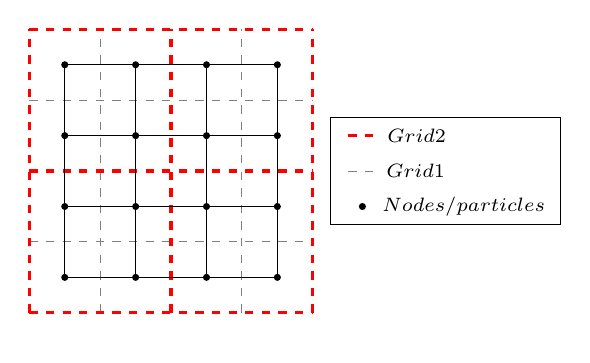
\begin{tikzpicture}[scale=0.9]
  \draw (0,0) --(3,0)--(3,3)--(0,3)--(0,0);
  \draw[white] (0.,0) -- (0,-0.8);
  %%% Grid 1
  \foreach \y in {-0.5,0.5,...,3.5} 
  \draw[dashed,gray] (-0.5,\y) -- (3.5,\y);
  \foreach \x in {-0.5,0.5,...,3.5} 
  \draw[dashed,gray] (\x,-0.5) -- (\x,3.5);
  %%% Grid 2
  \foreach \y in {-0.5,1.5,...,3.5} 
  \draw[dashed,Red,very thick] (-0.5,\y) -- (3.5,\y);
  \foreach \x in {-0.5,1.5,...,3.5} 
  \draw[dashed,Red,very thick] (\x,-0.5) -- (\x,3.5);
  \foreach \y in {0.,1.,...,3.} 
  \foreach \x in {0.,1.,...,3.} 
  \fill (\x,\y) circle(0.05);
  \foreach \y in {0.,1.,...,3.} 
  \draw (0,\y) -- (3.,\y);
  \foreach \x in {0.,1.,...,3.} 
  \draw (\x,0) -- (\x,3);
  \draw (3.75,0.75) rectangle (7.,2.25);
  \fill (4.2,1.) circle (0.05) node [right] {\scriptsize$ \: \: \text{Nodes / particles}$};
  \draw[dashed,gray] (4.,1.5) -- (4.4,1.5) node [right] {\scriptsize$\color{black} \text{Grid 1}$};
  \draw[dashed,very thick,Red] (4.,2.) -- (4.4,2.) node [right] {\scriptsize$\color{black} \text{Grid 2}$};
\end{tikzpicture}


%%% Local Variables:
%%% mode: latex
%%% TeX-master: "../manuscript"
%%% End:
}
  \caption{Geometry, loading and space discretizations used for the impact problem of a two-dimensional medium on a rigid wall. The initial velocity is set to $v_d=-200 \: m/s$.}
  \label{fig:PS_domain}
\end{figure}

The MPM and the DGMPM are compared to a $Q1$-finite element (bilinear approximation) solution coupled with a central difference explicit time integrator.
The domain is discretized such that material points are equivalent to finite element nodes: $l\times l \equiv 28 \times 28$ particles and nodes.
Moreover, two arbitrary grids are used for the particle-based methods so that either one or four material points lie in every cell according to the situations depicted in figure \ref{subfig:2d_meshes}.
This simulation enables comparisons between the numerical methods in spite of the lack of exact solution for that problem.

\subsubsection{Linear isotropic hardening material}
\label{sec:line-isotr-hard}

%The medium is first assumed to be made of the same material as before and comparisons in terms of the hydrostatic pressure $\bar{\sigma}=\frac{1}{3}\tens{\sigma}:\tens{I}$, where $\tens{\sigma}$ is the Cauchy stress tensor, and the cumulated plastic strain $p$ are shown in figure \ref{fig:PS_taylor}.
The medium is first assumed to be made of the same material as before and comparisons in terms of the longitudinal stress $\Pi_{11}$ and the cumulated plastic strain $p$ are shown in figure \ref{fig:PS_taylor}.
\begin{figure}[h!]
  \centering
  \subcaptionbox{Longitudinal stress \label{subfig:stress_comparison}}{\begin{tikzpicture}[scale=1]
  \begin{groupplot}[group style={group size=2 by 4,% columns by rows
      ylabels at=edge left, yticklabels at=edge left,
      horizontal sep=5.ex,
      vertical sep=2ex,},
    enlargelimits=0,
    xmin=0.,xmax=1., ymin=-0.,ymax=1.
    ,axis on top,scale only axis,width=0.18\linewidth
    ,xtick=\empty,ytick=\empty,
    colorbar style={
      title style={
        font=\normalsize,
        at={(1,.5)},
        anchor=north west
      },yticklabel style={font=\normalsize}
      ,at={(current axis.south east)},anchor=south west
    },colormap name=tol
    ]
    %% FIRST ROW (time 1 = 5.10e-4s)
    %%% RANGE -8.6e9 -- 0.57e9
    \nextgroupplot[title={$t=5.10\times 10^{-4} \:s$},ylabel={FEM}]\addplot graphics[xmin=0.,xmax=1., ymin=-0.,ymax=1.] {pngFigures/fem_stress1-crop.png};
    \nextgroupplot[title={$t=1.02\times 10^{-3} \:s$}]\addplot graphics[xmin=0.,xmax=1., ymin=-0.,ymax=1.] {pngFigures/fem_stress2-crop.png};

    \nextgroupplot[ylabel={MPM(1ppc)}]\addplot graphics[xmin=0.,xmax=1., ymin=-0.,ymax=1.] {pngFigures/mpm1ppc_stress1-crop.png};
    \nextgroupplot[]\addplot graphics[xmin=0.,xmax=1., ymin=-0.,ymax=1.] {pngFigures/mpm1ppc_stress2-crop.png};

    \nextgroupplot[ylabel={DGMPM(1ppc)}]\addplot graphics[xmin=0.,xmax=1., ymin=-0.,ymax=1.] {pngFigures/dgmpm1ppc_stress1-crop.png};
    \nextgroupplot[]\addplot graphics[xmin=0.,xmax=1., ymin=-0.,ymax=1.] {pngFigures/dgmpm1ppc_stress2-crop.png};
    

    \nextgroupplot[ylabel={DGMPM(4ppc)},colorbar horizontal,colorbar  style={
      title style={yshift=-1.5cm},
      title= {$\Pi_{11}\: (GPa)$},
      xtick={-8.6,0.56},
      xticklabels={-8.6,0.56},
    }]
    \addplot[scatter,scatter src=x,mark size=0.pt] coordinates {(-8.6,0.) (0.56,0)};% Fake extreme values to fix scale
    \addplot graphics[xmin=0.,xmax=1., ymin=-0.,ymax=1.] {pngFigures/dgmpm4ppc_stress1-crop.png};
    \nextgroupplot[colorbar horizontal,colorbar  style={
      title style={yshift=-1.5cm},
      title= {$\Pi_{11}\: (GPa)$},
      xtick={-3,7.6},
      xticklabels={-3,7.6},
    }]
    \addplot[scatter,scatter src=x,mark size=0.pt] coordinates {(-3.,0.) (7.6,0)};% Fake extreme values to fix scale
    \addplot graphics[xmin=0.,xmax=1., ymin=-0.,ymax=1.] {pngFigures/dgmpm4ppc_stress2-crop.png};
    
  \end{groupplot}
\end{tikzpicture}



%%% Local Variables:
%%% mode: latex
%%% TeX-master: "../manuscript"
%%% End:
}\qquad
  %\subcaptionbox{Hydrostatic pressure \label{subfig:press_comparison}}{\begin{tikzpicture}[scale=1]
  \begin{groupplot}[group style={group size=2 by 4,% columns by rows
      ylabels at=edge left, yticklabels at=edge left,
      horizontal sep=5.ex,
      vertical sep=2ex,},
    enlargelimits=0,
    xmin=0.,xmax=1., ymin=-0.,ymax=1.
    ,axis on top,scale only axis,width=0.18\linewidth
    ,xtick=\empty,ytick=\empty,
    colorbar style={
      title style={
        font=\normalsize,
        at={(1,.5)},
        anchor=north west
      },yticklabel style={font=\normalsize}
      ,at={(current axis.south east)},anchor=south west
    },colormap name=tol
    ]
    %% FIRST ROW (time 1 = 5.10e-4s)
    %%% RANGE -8.6e9 -- 0.57e9
    \nextgroupplot[title={$t=5.10\times 10^{-4} \:s$},ylabel={FEM}]\addplot graphics[xmin=0.,xmax=1., ymin=-0.,ymax=1.] {pngFigures/fem_press1-crop.png};
    \nextgroupplot[title={$t=1.02\times 10^{-3} \:s$}]\addplot graphics[xmin=0.,xmax=1., ymin=-0.,ymax=1.] {pngFigures/fem_press2-crop.png};

    \nextgroupplot[ylabel={MPM(1ppc)}]\addplot graphics[xmin=0.,xmax=1., ymin=-0.,ymax=1.] {pngFigures/mpm_press1-crop.png};
    \nextgroupplot[]\addplot graphics[xmin=0.,xmax=1., ymin=-0.,ymax=1.] {pngFigures/mpm_press2-crop.png};

    \nextgroupplot[ylabel={DGMPM(1ppc)}]\addplot graphics[xmin=0.,xmax=1., ymin=-0.,ymax=1.] {pngFigures/dgmpm1ppc_press1-crop.png};
    \nextgroupplot[]\addplot graphics[xmin=0.,xmax=1., ymin=-0.,ymax=1.] {pngFigures/dgmpm1ppc_press2-crop.png};
    

    \nextgroupplot[ylabel={DGMPM(4ppc)},colorbar horizontal,colorbar  style={
      title style={yshift=-1.5cm},
      title= {$\bar{\sigma}\: (GPa)$},
      xtick={-8.,1.2},
      xticklabels={-8,1.2},
    }]
    \addplot[scatter,scatter src=x,mark size=0.pt] coordinates {(-8.,0.) (1.2,0)};% Fake extreme values to fix scale
    \addplot graphics[xmin=0.,xmax=1., ymin=-0.,ymax=1.] {pngFigures/dgmpm4ppc_press1-crop.png};
    \nextgroupplot[colorbar horizontal,colorbar  style={
      title style={yshift=-1.5cm},
      title= {$\bar{\sigma}\: (GPa)$},
      xtick={-2.1,7.9},
      xticklabels={-2.1,7.9},
    }]
    \addplot[scatter,scatter src=x,mark size=0.pt] coordinates {(-2.1,0.) (7.9,0)};% Fake extreme values to fix scale
    \addplot graphics[xmin=0.,xmax=1., ymin=-0.,ymax=1.] {pngFigures/dgmpm4ppc_press2-crop.png};
    
  \end{groupplot}
\end{tikzpicture}



%%% Local Variables:
%%% mode: latex
%%% TeX-master: "../manuscript"
%%% End:
}\qquad
  \subcaptionbox{Cumulated plastic strain \label{subfig:epls_comparison}}{\begin{tikzpicture}[scale=1]
  \begin{groupplot}[group style={group size=2 by 4,% columns by rows
      ylabels at=edge left, yticklabels at=edge left,
      horizontal sep=5.ex,
      vertical sep=2ex,},
    enlargelimits=0,
    xmin=0.,xmax=1., ymin=-0.,ymax=1.
    ,axis on top,scale only axis,xtick=\empty,ytick=\empty,width=0.18\linewidth,
    colorbar style={
      title style={
        font=\normalsize,
        at={(1,.5)},
        anchor=north west
      },yticklabel style={font=\normalsize}
      ,at={(current axis.south east)},anchor=south west
    },colormap name=tol]
    %% FIRST ROW (time 1 = 5.10e-4s)
    %%% RANGE -8.6e9 -- 0.57e9
    \nextgroupplot[title={$t=5.10\times 10^{-4} \:s$},ylabel={FEM}]\addplot graphics[xmin=0.,xmax=1., ymin=-0.,ymax=1.] {pngFigures/fem_epeq1-crop.png};
    \nextgroupplot[title={$t=1.02\times 10^{-3} \:s$}]\addplot graphics[xmin=0.,xmax=1., ymin=-0.,ymax=1.] {pngFigures/fem_epeq2-crop.png};

    \nextgroupplot[ylabel={MPM}]\addplot graphics[xmin=0.,xmax=1., ymin=-0.,ymax=1.] {pngFigures/mpm_epeq1-crop.png};
    \nextgroupplot[]\addplot graphics[xmin=0.,xmax=1., ymin=-0.,ymax=1.] {pngFigures/mpm_epeq2-crop.png};

    \nextgroupplot[ylabel={DGMPM--1ppc}]\addplot graphics[xmin=0.,xmax=1., ymin=-0.,ymax=1.] {pngFigures/dgmpm1ppc_epeq1-crop.png};
    \nextgroupplot[]\addplot graphics[xmin=0.,xmax=1., ymin=-0.,ymax=1.] {pngFigures/dgmpm1ppc_epeq2-crop.png};
    

    \nextgroupplot[ylabel={DGMPM--4ppc},colorbar horizontal,colorbar  style={
      title style={yshift=-1.5cm},
      title= {$p$},
      xtick={0,.15},
      xticklabels={0,0.15},
    }]
    \addplot[scatter,scatter src=x,mark size=0.pt] coordinates {(0,0.) (0.15,0)};% Fake extreme values to fix scale
    \addplot graphics[xmin=0.,xmax=1., ymin=-0.,ymax=1.] {pngFigures/dgmpm4ppc_epeq1-crop.png};
    \nextgroupplot[colorbar horizontal,colorbar  style={
      title style={yshift=-1.5cm},
      title= {$p$},
      xtick={0.,0.16},
      xticklabels={0,0.16},
    }]
    \addplot[scatter,scatter src=x,mark size=0.pt] coordinates {(0.,0.) (0.16,0)};% Fake extreme values to fix scale
    \addplot graphics[xmin=0.,xmax=1., ymin=-0.,ymax=1.] {pngFigures/dgmpm4ppc_epeq2-crop.png};
    
  \end{groupplot}
\end{tikzpicture}



%%% Local Variables:
%%% mode: latex
%%% TeX-master: "../manuscript"
%%% End:
}
  %\caption{Isovalues of the hydrostatic pressure $\bar{\sigma}$ and cumulated plastic strain in a two-dimensional hyperelastic-plastic solids impacting a rigid wall under plane strain. Comparison of FEM (CFL=0.9), MPM (CFL=0.7) and DGMPM solutions using either one particle per cell (CFL=1) or four particles per cell (CFL=0.4).}
  \caption{Isovalues of the PK1 stress component $\Pi_{11}$ and cumulated plastic strain in a two-dimensional hyperelastic-plastic solids impacting a rigid wall under plane strain. Comparison of FEM (CFL=0.9), MPM (CFL=0.7) and DGMPM solutions using either one particle per cell (CFL=1) or four particles per cell (CFL=0.4).}
  \label{fig:PS_taylor}
\end{figure}
Notice that a mesh is reconstructed for MPM and DGMPM results for visualization purpose, and that the comparisons are made in the deformed configuration for two time steps that correspond to the incident and reflected pressure waves.

Before the reflection of the pressure wave, the occurence of spurious oscillations in MPM and FEM solutions, though much slighter in the latter, and of numerical diffusion in the DGMPM(4ppc) one, lead to different assessment of fields.
In addition to the stress peaks occuring in the MPM solution in the bottom part of the domain, a checkerboard structure can be seen upstream.
Recall that the MPM(1ppc) is equivalent to a reduced-integrated FEM so that these oscillations are not related to volumetric locking.
Note moreover that no signs of such a locking appears in the FEM solution, it then seems that the loading conditions considered do not make the deformation incompressibility-dominated.
Then, figure \ref{subfig:epls_comparison} shows that the numerical cumulated plastic strains have globally the same shape but different extreme values.
% Figure \ref{fig:PS_taylor_pressure} shows the isovalues of the hydrostatic pressure $\bar{\sigma}=\frac{1}{3}\tens{\sigma}:\tens{I}$, where $\tens{\sigma}$ is the Cauchy stress tensor, in the two-dimensional medium for all the numerical schemes at time $t= 5.10 \times 10^{-4}\: s$.
% It can thus be seen that the oscillations in MPM solution is not due to volumetric locking since the characteristic pattern of that numerical artifact is not visible.
% Moreover, it is worth noticing that no numerical method yields such a locking for the loading conditions considered.
% \begin{figure}[h!]
%   \centering
%   \input{pgfFigures/press_comparison2}
%   \caption{Isovalues of the numerical hydrostatic pressures $\bar{\sigma}$ at time $t= 5.10 \times 10^{-4}\: s$.}
%   \label{fig:PS_taylor_pressure}
% \end{figure}

Next, the incident wave reflects on the right end of the solid as a tensile wave so that the bottom part of that boundary starts moving rightward.
After that reflection, similar observations can be made on the MPM and the DGMPM(4ppc) stress solutions, that is, significant oscillations and numerical diffusion respectively.
Moreover, although the FEM and DGMPM(1ppc) stresss are quite similar before the reflection, it is no longer the case after the passage of the tensile wave so that the FEM solution exhibits a maximum value that is higher than the DGMPM one.
On the other hand, the plasticity continues propagating within the domain and no significant difference appears in the numerical cumulated plastic strains.
At that time, it can also be seen that the shapes of the solid domain are quite similar, even though DGMPM solutions leads to a slightly lower vertical displacement of the top left corner of the square.

We now propose to look at the above results in more details.
Figures \ref{fig:bottom_line} and \ref{fig:left_line} show the evolution of longitudinal stress and cumulated plastic strain along the bottom and left ends of the domain respectively for the same time steps as before.
First, it can be seen in figure \ref{subfig:bottom1} that the incident wave is described with different levels of sharpness by the numerical schemes.
% Note however that no elastic predictor is seen in the stress profiles in contrast to the one-dimensional problem studied above.
\begin{figure}[h!]
  \centering
  {\phantomsubcaption{\label{subfig:bottom1}}}
  {\phantomsubcaption{\label{subfig:bottom2}}}
  \begin{tikzpicture}
  \begin{groupplot}[group style={group size=2 by 2, % 3 columns 2 rows
      ylabels at=edge left, yticklabels at=edge left,horizontal sep=2.ex,vertical sep=5.ex,
      xticklabels at=edge bottom,xlabels at=edge bottom},
    ymajorgrids=true,xmajorgrids=true,
    axis on top,scale only axis,width=0.425\linewidth,
    height=0.25\linewidth,
    every x tick scale label/.style={at={(xticklabel* cs:1.05,0.75cm)},anchor=near yticklabel},
    every y tick scale label/.style={at={(yticklabel* cs:1.05,-.9cm)},anchor=near yticklabel}]
    
    %%%%%%%%%%%%%%%%%%%% 
    % ============================== Stress Line
    % t1 
    \nextgroupplot[ylabel=$\Pi_{11} \:(Pa)$,title={(a) $t = 5.10 \times 10^{-4}\: s$},ymin=-1.e10,ymax=7.25e9]
    \addplot[Orange,thick,mark=*,mark repeat=2] table[x=Points:0,y=Piola_Stress:0] {csvFiles/fem_bottom1.csv};
    \addplot[Red,thick,mark=square,only marks] table[x=Points:0,y=Piola:0] {csvFiles/mpm_bottom1.csv};
    \addplot[black!60,thick,mark=o,only marks] table[x=Points:0,y=Piola:0] {csvFiles/mpm4ppc_bottom1.csv};
    \addplot[Blue,thick,mark=asterisk,only marks,mark size=3pt] table[x=Points:0,y=PK1:0] {csvFiles/dgmpm1ppc_bottom1.csv};
    \addplot[Purple,thick,mark=x,only marks,mark size=3pt,mark repeat=2] table[x=Points:0,y=PK1:0] {csvFiles/dgmpm4ppc_bottom1.csv};
    
    % t2 
    \nextgroupplot[title={(b) $t = 1.02 \times 10^{-3}\: s$},ymin=-1.e10,ymax=7.25e9%,ymin=-7.5e9,ymax=100.e9,ytick scale label code/.code={},legend style={at={($(0.75,-0.4)+(0.9cm,0.6cm)$)},legend columns=3}
    ]
    \addplot[Orange,thick,mark=*,mark repeat=2] table[x=Points:0,y=Piola_Stress:0] {csvFiles/fem_bottom2.csv};
    \addplot[Red,thick,mark=square,only marks] table[x=Points:0,y=Piola:0] {csvFiles/mpm_bottom2.csv};
    \addplot[black!60,thick,mark=o,only marks] table[x=Points:0,y=Piola:0] {csvFiles/mpm4ppc_bottom2.csv};
    \addplot[Blue,thick,mark=asterisk,only marks,mark size=3pt] table[x=Points:0,y=PK1:0] {csvFiles/dgmpm1ppc_bottom2.csv};
    \addplot[Purple,thick,mark=x,only marks,mark size=3pt,mark repeat=2] table[x=Points:0,y=PK1:0] {csvFiles/dgmpm4ppc_bottom2.csv};


    % ============================== Cumulated plastic strain Line
    % t1 
    \nextgroupplot[ylabel=$p$,xlabel=$x_1 \: (m)$,ymin=0.,ymax=9.e-2%,ymin=-7.5e9,ymax=100.e9,ytick scale label code/.code={}
    ]
    \addplot[Orange,thick,mark=*,mark repeat=2] table[x=Points:0,y=Equivalent_Plastic_Strain] {csvFiles/fem_bottom1.csv};
    \addplot[Red,thick,mark=square,only marks] table[x=Points:0,y=epeq] {csvFiles/mpm_bottom1.csv};
    \addplot[black!60,thick,mark=o,only marks] table[x=Points:0,y=epeq] {csvFiles/mpm4ppc_bottom1.csv};
    \addplot[Blue,thick,mark=asterisk,only marks,mark size=3pt] table[x=Points:0,y=epeq] {csvFiles/dgmpm1ppc_bottom1.csv};
    \addplot[Purple,thick,mark=x,only marks,mark size=3pt,mark repeat=2] table[x=Points:0,y=epeq] {csvFiles/dgmpm4ppc_bottom1.csv};
    
    % t2
    \nextgroupplot[legend style={at={($(0.75,-0.35)+(0.2cm,0.35cm)$)},legend columns=5},xlabel=$x_1 \: (m)$,ymin=0.,ymax=9.e-2%,ymin=-7.5e9,ymax=100.e9,ytick scale label code/.code={}
    ]
    \addplot[Orange,thick,mark=*,mark repeat=2] table[x=Points:0,y=Equivalent_Plastic_Strain] {csvFiles/fem_bottom2.csv};
    \addplot[Red,thick,mark=square,only marks] table[x=Points:0,y=epeq] {csvFiles/mpm_bottom2.csv};
    \addplot[black!60,thick,mark=o,only marks] table[x=Points:0,y=epeq] {csvFiles/mpm4ppc_bottom2.csv};
    \addplot[Blue,thick,mark=asterisk,only marks,mark size=3pt] table[x=Points:0,y=epeq] {csvFiles/dgmpm1ppc_bottom2.csv};
    \addplot[Purple,thick,mark=x,only marks,mark size=3pt,mark repeat=2] table[x=Points:0,y=epeq] {csvFiles/dgmpm4ppc_bottom2.csv};

    \addlegendentry{fem \:}
    \addlegendentry{mpm (1ppc) \:}
    \addlegendentry{mpm (4ppc) \:}
    \addlegendentry{dgmpm (1ppc) \:}
    \addlegendentry{dgmpm (4ppc) \:}
    
    
  \end{groupplot}
\end{tikzpicture}



%%% Local Variables:
%%% mode: latex
%%% TeX-master: "../manuscript"
%%% End:

  \caption{Comparison of the longitudinal stress component and cumulated plastic strain along the bottom boundary of the domain at two times.}
  \label{fig:bottom_line}
\end{figure}
Then, the figure also shows the oscillations in the MPM stress solution already mentioned.
Moreover, the superimposition of the stresses resulting from MPM computations using 1ppc or 4ppc shows that refining the particles discretization does not allow the removal of the numerical noise.
%As a consequence, the numerical cumulated plastic strains near the wave front are rather different since the solutions of particle-based methods are ahead of the FEM one.
In addition, it can be seen that the plastic strain plateau is not similarly computed by all the numerical methods and that smoother profiles are obtained with the particle-based approaches. 
Upstream the plastic front, the MPM(4ppc) plastic strain exhibits some peaks while this computed with the MPM(1ppc) is closer to the finite element solution.
On the other hand, the two DGMPM results are close from one to another on the plastic plateau.

After the reflection (figure \ref{subfig:bottom2}), the stress profiles are much more different. 
The MPM still yields oscillating solutions regardless of the space discretization used, and DGMPM results are smoother than the other.
Once Again, the FEM leads to a sharper resolution of the reflected elastic pressure wave.
Furthermore, the MPM cumulated plastic strain curves oscillate around the FEM one which, in turn, is above these computed with the DGMPM.

The previous observations are even more significant when looking at the evolution of fields along the left end of the square (figure \ref{fig:left_line}).
In figure \ref{subfig:left1}, FEM and DGMPM stress profiles show good agreement while spurious oscillations pollute MPM ones. 
Although FEM and DGMPM stresses are similar, it is not the case for the cumulated plastic strains for which the numerical results differ more.
Thus, the MPM yields the highest values of cumulated plastic strain at the top left corner of the domain.
The results depicted at the subsequent time show tremendous oscillations in the MPM(1ppc) solution for which the longitudinal stress varies roughly from $-7 \: GPa$ to $1 \: GPa$ in the bottom part of the left boundary.
These oscillations are reduced, though not completely removed, in the MPM(4ppc) results. 
On the other hand, DGMPM and FEM solutions no longer fit.
\begin{figure}[h!]
  \centering
  {\phantomsubcaption{\label{subfig:left1}}}
  {\phantomsubcaption{\label{subfig:left2}}}
  \begin{tikzpicture}
  \begin{groupplot}[group style={group size=2 by 2, % 3 columns 2 rows
      ylabels at=edge left, yticklabels at=edge left,horizontal sep=2.ex,vertical sep=3.ex,
      xticklabels at=edge bottom,xlabels at=edge bottom},
    ymajorgrids=true,xmajorgrids=true,
    axis on top,scale only axis,width=0.425\linewidth, every x tick scale label/.style={at={(xticklabel* cs:1.05,0.75cm)},anchor=near yticklabel},
    every y tick scale label/.style={at={(yticklabel* cs:1.05,-0.9cm)},anchor=near yticklabel}]
    
    %%%%%%%%%%%%%%%%%%%% 
    % ============================== Stress Line
    % t1 
    \nextgroupplot[ylabel=$\Pi_{11} \:(Pa)$,title={(a) $t = 5.10 \times 10^{-4}\: s$},ymin=-8.5e9,ymax=2.e9]
    \addplot[Orange,thick,mark=*,mark repeat=2] table[x=Points:1,y=Piola_Stress:0] {csvFiles/fem_left1.csv};
    \addplot[Red,thick,mark=square,only marks] table[x=Points:1,y=Piola:0] {csvFiles/mpm_left1.csv};
    \addplot[black!60,thick,mark=o,only marks] table[x=Points:1,y=Piola:0] {csvFiles/mpm4ppc_left1.csv};
    \addplot[Blue,thick,mark=asterisk,only marks,mark size=3pt] table[x=Points:1,y=PK1:0] {csvFiles/dgmpm1ppc_left1.csv};
    \addplot[Purple,thick,mark=x,only marks,mark size=3pt,mark repeat=2] table[x=Points:1,y=PK1:0] {csvFiles/dgmpm4ppc_left1.csv};
    
    % t2 
    \nextgroupplot[title={(b) $t = 1.02 \times 10^{-3}\: s$},ymin=-8.5e9,ymax=2.e9%,ymin=-7.5e9,ymax=100.e9,ytick scale label code/.code={},legend style={at={($(0.75,-0.4)+(0.9cm,0.6cm)$)},legend columns=3}
    ]
    \addplot[Orange,thick,mark=*,mark repeat=2] table[x=Points:1,y=Piola_Stress:0] {csvFiles/fem_left2.csv};
    \addplot[Red,thick,mark=square,only marks] table[x=Points:1,y=Piola:0] {csvFiles/mpm_left2.csv};
    \addplot[black!60,thick,mark=o,only marks] table[x=Points:1,y=Piola:0] {csvFiles/mpm4ppc_left2.csv};
    \addplot[Blue,thick,mark=asterisk,only marks,mark size=3pt] table[x=Points:1,y=PK1:0] {csvFiles/dgmpm1ppc_left2.csv};
    \addplot[Purple,thick,mark=x,only marks,mark size=3pt,mark repeat=2] table[x=Points:1,y=PK1:0] {csvFiles/dgmpm4ppc_left2.csv};


    % ============================== Cumulated plastic strain Line
    % t1 
    \nextgroupplot[ylabel=$p$,xlabel=$y \: (m)$,ymin=2.e-2,ymax=1.8e-1%,ymin=-7.5e9,ymax=100.e9,ytick scale label code/.code={}
    ]
    \addplot[Orange,thick,mark=*,mark repeat=2] table[x=Points:1,y=Equivalent_Plastic_Strain] {csvFiles/fem_left1.csv};
    \addplot[Red,thick,mark=square,only marks] table[x=Points:1,y=epeq] {csvFiles/mpm_left1.csv};
    \addplot[black!60,thick,mark=o,only marks] table[x=Points:1,y=epeq] {csvFiles/mpm4ppc_left1.csv};
    \addplot[Blue,thick,mark=asterisk,only marks,mark size=3pt] table[x=Points:1,y=epeq] {csvFiles/dgmpm1ppc_left1.csv};
    \addplot[Purple,thick,mark=x,only marks,mark size=3pt,mark repeat=2] table[x=Points:1,y=epeq] {csvFiles/dgmpm4ppc_left1.csv};
    
    % t2
    \nextgroupplot[legend style={at={($(0.75,-0.35)+(0.cm,1cm)$)},legend columns=5},xlabel=$y \: (m)$,ymin=2.e-2,ymax=1.8e-1%,ymin=-7.5e9,ymax=100.e9,ytick scale label code/.code={}
    ]
    \addplot[Orange,thick,mark=*,mark repeat=2] table[x=Points:1,y=Equivalent_Plastic_Strain] {csvFiles/fem_left2.csv};
    \addplot[black!60,thick,mark=o,only marks] table[x=Points:1,y=epeq] {csvFiles/mpm_left2.csv};
    \addplot[Red,thick,mark=square,only marks] table[x=Points:1,y=epeq] {csvFiles/mpm4ppc_left2.csv};
    \addplot[Blue,thick,mark=asterisk,only marks,mark size=3pt] table[x=Points:1,y=epeq] {csvFiles/dgmpm1ppc_left2.csv};
    \addplot[Purple,thick,mark=x,only marks,mark size=3pt,mark repeat=2] table[x=Points:1,y=epeq] {csvFiles/dgmpm4ppc_left2.csv};

    \addlegendentry{fem \:}
    \addlegendentry{mpm (1ppc) \:}
    \addlegendentry{mpm (4ppc) \:}
    \addlegendentry{dgmpm (1ppc) \:}
    \addlegendentry{dgmpm (4ppc) \:}
    
    
  \end{groupplot}
\end{tikzpicture}



%%% Local Variables:
%%% mode: latex
%%% TeX-master: "../manuscript"
%%% End:

  \caption{Comparison of the longitudinal stress component and cumulated plastic strain along the left boundary of the domain at two times.}
  \label{fig:left_line}
\end{figure}
It appears that the stress curve corresponding to the latter is bounded by these of the DGMPM(4ppc) and DGMPM(1ppc), the lower bound being given by the single particle space discretization.
At last, the cumulated plastic strain curves show similar behaviors to those of the previous time step except close to the bottom left corner of the domain.
In that region, the plastic flow developed differently depending on the numerical solution considered.
Both DGMPM curves are below that computed with the FEM while the profiles resulting from MPM computations are less regular than the others.

\subsubsection{Non-linear isotropic hardening material}
\label{sec:non-linear-hardening}
The previous problem is now considered in a material whose isotropic hardening follows a power law, for which the same comparisons as before are made. 

\begin{figure}[h!]
  \centering
  %\subcaptionbox{Stress \label{subfig:stress_comparison}}{\begin{tikzpicture}[scale=1]
  \begin{groupplot}[group style={group size=2 by 4,% columns by rows
      ylabels at=edge left, yticklabels at=edge left,
      horizontal sep=5.ex,
      vertical sep=2ex,},
    enlargelimits=0,
    xmin=0.,xmax=1., ymin=-0.,ymax=1.
    ,axis on top,scale only axis,width=0.18\linewidth
    ,xtick=\empty,ytick=\empty,
    colorbar style={
      title style={
        font=\normalsize,
        at={(1,.5)},
        anchor=north west
      },yticklabel style={font=\normalsize}
      ,at={(current axis.south east)},anchor=south west
    },colormap name=tol
    ]
    %% FIRST ROW (time 1 = 5.10e-4s)
    %%% RANGE -8.6e9 -- 0.57e9
    \nextgroupplot[title={$t=5.10\times 10^{-4} \:s$},ylabel={FEM}]\addplot graphics[xmin=0.,xmax=1., ymin=-0.,ymax=1.] {pngFigures/fem_stress1-crop.png};
    \nextgroupplot[title={$t=1.02\times 10^{-3} \:s$}]\addplot graphics[xmin=0.,xmax=1., ymin=-0.,ymax=1.] {pngFigures/fem_stress2-crop.png};

    \nextgroupplot[ylabel={MPM(1ppc)}]\addplot graphics[xmin=0.,xmax=1., ymin=-0.,ymax=1.] {pngFigures/mpm1ppc_stress1-crop.png};
    \nextgroupplot[]\addplot graphics[xmin=0.,xmax=1., ymin=-0.,ymax=1.] {pngFigures/mpm1ppc_stress2-crop.png};

    \nextgroupplot[ylabel={DGMPM(1ppc)}]\addplot graphics[xmin=0.,xmax=1., ymin=-0.,ymax=1.] {pngFigures/dgmpm1ppc_stress1-crop.png};
    \nextgroupplot[]\addplot graphics[xmin=0.,xmax=1., ymin=-0.,ymax=1.] {pngFigures/dgmpm1ppc_stress2-crop.png};
    

    \nextgroupplot[ylabel={DGMPM(4ppc)},colorbar horizontal,colorbar  style={
      title style={yshift=-1.5cm},
      title= {$\Pi_{11}\: (GPa)$},
      xtick={-8.6,0.56},
      xticklabels={-8.6,0.56},
    }]
    \addplot[scatter,scatter src=x,mark size=0.pt] coordinates {(-8.6,0.) (0.56,0)};% Fake extreme values to fix scale
    \addplot graphics[xmin=0.,xmax=1., ymin=-0.,ymax=1.] {pngFigures/dgmpm4ppc_stress1-crop.png};
    \nextgroupplot[colorbar horizontal,colorbar  style={
      title style={yshift=-1.5cm},
      title= {$\Pi_{11}\: (GPa)$},
      xtick={-3,7.6},
      xticklabels={-3,7.6},
    }]
    \addplot[scatter,scatter src=x,mark size=0.pt] coordinates {(-3.,0.) (7.6,0)};% Fake extreme values to fix scale
    \addplot graphics[xmin=0.,xmax=1., ymin=-0.,ymax=1.] {pngFigures/dgmpm4ppc_stress2-crop.png};
    
  \end{groupplot}
\end{tikzpicture}



%%% Local Variables:
%%% mode: latex
%%% TeX-master: "../manuscript"
%%% End:
}\qquad
  \subcaptionbox{Pressure \label{subfig:press_comparison_NL}}{\begin{tikzpicture}[scale=1]
  \begin{groupplot}[group style={group size=2 by 4,% columns by rows
      ylabels at=edge left, yticklabels at=edge left,
      horizontal sep=5.ex,
      vertical sep=2ex,},
    enlargelimits=0,
    xmin=0.,xmax=1., ymin=-0.,ymax=1.
    ,axis on top,scale only axis,width=0.18\linewidth
    ,xtick=\empty,ytick=\empty,
    colorbar style={
      title style={
        font=\normalsize,
        at={(1,.5)},
        anchor=north west
      },yticklabel style={font=\normalsize}
      ,at={(current axis.south east)},anchor=south west
    },colormap name=tol
    ]
    %% FIRST ROW (time 1 = 5.10e-4s)
    %%% RANGE -8.6e9 -- 0.57e9
    \nextgroupplot[title={$t=5.10\times 10^{-4} \:s$},ylabel={FEM}]\addplot graphics[xmin=0.,xmax=1., ymin=-0.,ymax=1.] {pngFigures/NLhardening/fem_press1-crop.png};
    \nextgroupplot[title={$t=1.02\times 10^{-3} \:s$}]\addplot graphics[xmin=0.,xmax=1., ymin=-0.,ymax=1.] {pngFigures/NLhardening/fem_press2-crop.png};

    \nextgroupplot[ylabel={MPM(1ppc)}]\addplot graphics[xmin=0.,xmax=1., ymin=-0.,ymax=1.] {pngFigures/NLhardening/mpm_press1-crop.png};
    \nextgroupplot[]\addplot graphics[xmin=0.,xmax=1., ymin=-0.,ymax=1.] {pngFigures/NLhardening/mpm_press2-crop.png};

    \nextgroupplot[ylabel={DGMPM(1ppc)}]\addplot graphics[xmin=0.,xmax=1., ymin=-0.,ymax=1.] {pngFigures/NLhardening/dgmpm1ppc_press1-crop.png};
    \nextgroupplot[]\addplot graphics[xmin=0.,xmax=1., ymin=-0.,ymax=1.] {pngFigures/NLhardening/dgmpm1ppc_press2-crop.png};
    

    \nextgroupplot[ylabel={DGMPM(4ppc)},colorbar horizontal,colorbar  style={
      title style={yshift=-1.5cm},
      title= {$\bar{\sigma}\: (GPa)$},
      xtick={-8.1,2.3},
      xticklabels={-8.1,2.3},
    }]
    \addplot[scatter,scatter src=x,mark size=0.pt] coordinates {(-8.1,0.) (2.3,0)};% Fake extreme values to fix scale
    \addplot graphics[xmin=0.,xmax=1., ymin=-0.,ymax=1.] {pngFigures/NLhardening/dgmpm4ppc_press1-crop.png};
    \nextgroupplot[colorbar horizontal,colorbar  style={
      title style={yshift=-1.5cm},
      title= {$\bar{\sigma}\: (GPa)$},
      xtick={-2.1,7.9},
      xticklabels={-2.1,7.9},
    }]
    \addplot[scatter,scatter src=x,mark size=0.pt] coordinates {(-2.1,0.) (7.9,0)};% Fake extreme values to fix scale
    \addplot graphics[xmin=0.,xmax=1., ymin=-0.,ymax=1.] {pngFigures/NLhardening/dgmpm4ppc_press2-crop.png};
    
  \end{groupplot}
\end{tikzpicture}



%%% Local Variables:
%%% mode: latex
%%% TeX-master: "../manuscript"
%%% End:
}\qquad
  \subcaptionbox{Cumulated plastic strain \label{subfig:epls_comparison_NL}}{\begin{tikzpicture}[scale=1]
  \begin{groupplot}[group style={group size=2 by 4,% columns by rows
      ylabels at=edge left, yticklabels at=edge left,
      horizontal sep=5.ex,
      vertical sep=2ex,},
    enlargelimits=0,
    xmin=0.,xmax=1., ymin=-0.,ymax=1.
    ,axis on top,scale only axis,xtick=\empty,ytick=\empty,width=0.18\linewidth,
    colorbar style={
      title style={
        font=\normalsize,
        at={(1,.5)},
        anchor=north west
      },yticklabel style={font=\normalsize}
      ,at={(current axis.south east)},anchor=south west
    },colormap name=tol]
    %% FIRST ROW (time 1 = 5.10e-4s)
    %%% RANGE -8.6e9 -- 0.57e9
    \nextgroupplot[title={$t=5.10\times 10^{-4} \:s$},ylabel={FEM}]\addplot graphics[xmin=0.,xmax=1., ymin=-0.,ymax=1.] {pngFigures/NLhardening/fem_epeq1-crop.png};
    \nextgroupplot[title={$t=1.02\times 10^{-3} \:s$}]\addplot graphics[xmin=0.,xmax=1., ymin=-0.,ymax=1.] {pngFigures/NLhardening/fem_epeq2-crop.png};

    \nextgroupplot[ylabel={MPM(1ppc)}]\addplot graphics[xmin=0.,xmax=1., ymin=-0.,ymax=1.] {pngFigures/NLhardening/mpm_epeq1-crop.png};
    \nextgroupplot[]\addplot graphics[xmin=0.,xmax=1., ymin=-0.,ymax=1.] {pngFigures/NLhardening/mpm_epeq2-crop.png};

    \nextgroupplot[ylabel={DGMPM(1ppc)}]\addplot graphics[xmin=0.,xmax=1., ymin=-0.,ymax=1.] {pngFigures/NLhardening/dgmpm1ppc_epeq1-crop.png};
    \nextgroupplot[]\addplot graphics[xmin=0.,xmax=1., ymin=-0.,ymax=1.] {pngFigures/NLhardening/dgmpm1ppc_epeq2-crop.png};
    

    \nextgroupplot[ylabel={DGMPM(4ppc)},colorbar horizontal,colorbar  style={
      title style={yshift=-1.5cm},
      title= {$p$},
      xtick={0,.2},
      xticklabels={0,0.2},
    }]
    \addplot[scatter,scatter src=x,mark size=0.pt] coordinates {(0,0.) (0.2,0)};% Fake extreme values to fix scale
    \addplot graphics[xmin=0.,xmax=1., ymin=-0.,ymax=1.] {pngFigures/NLhardening/dgmpm4ppc_epeq1-crop.png};
    \nextgroupplot[colorbar horizontal,colorbar  style={
      title style={yshift=-1.5cm},
      title= {$p$},
      xtick={0.,0.25},
      xticklabels={0,0.25},
    }]
    \addplot[scatter,scatter src=x,mark size=0.pt] coordinates {(0.,0.) (0.25,0)};% Fake extreme values to fix scale
    \addplot graphics[xmin=0.,xmax=1., ymin=-0.,ymax=1.] {pngFigures/NLhardening/dgmpm4ppc_epeq2-crop.png};
    
  \end{groupplot}
\end{tikzpicture}



%%% Local Variables:
%%% mode: latex
%%% TeX-master: "../manuscript"
%%% End:
}
  \caption{Isovalues of the hydrostatic pressure $\bar{\sigma}$ and the cumulated plastic strain in a two-dimensional hyperelastic-plastic solids impacting a rigid wall under plane strain. Comparison of FEM (CFL=0.9), MPM (CFL=0.7) and DGMPM solutions using either one particle per cell (CFL=1) or four particles per cell (CFL=0.4).}
  \label{fig:PS_taylor_NL}
\end{figure}

%\review{Il y a un point bizzare dans la solution DGMPM (1ppc) de $p$}

% \begin{figure}[h!]
%   \centering
%   {\phantomsubcaption{\label{subfig:bottom1}}}
%   {\phantomsubcaption{\label{subfig:bottom2}}}
%   \begin{tikzpicture}
  \begin{groupplot}[group style={group size=2 by 2, % 3 columns 2 rows
      ylabels at=edge left, yticklabels at=edge left,horizontal sep=2.ex,vertical sep=5.ex,
      xticklabels at=edge bottom,xlabels at=edge bottom},
    ymajorgrids=true,xmajorgrids=true,
    axis on top,scale only axis,width=0.45\linewidth,height=0.25\linewidth,
    every x tick scale label/.style={at={(xticklabel* cs:1.05,0.75cm)},anchor=near yticklabel},
    % every y tick scale label/.style={at={(yticklabel* cs:1.15,-.9cm)},anchor=near yticklabel}
    ]
    
    %%%%%%%%%%%%%%%%%%%% 
    % ============================== Stress Line
    % t1 
    \nextgroupplot[ylabel=$\Pi_{11} \:(Pa)$,title={(a) $t = 1.9 \times 10^{-4}\: s$},ymin=-.25e9,ymax=2e10]
    \addplot[Orange,thick,mark=*,mark repeat=2] table[x=Points:0,y=Piola_Stress:0] {csvFiles/NLhardening/fem_bottom1.csv};
    \addplot[Red,thick,mark=square,only marks] table[x=Points:0,y=Piola:0] {csvFiles/NLhardening/mpm_bottom1.csv};
    \addplot[black!60,thick,mark=o,only marks] table[x=Points:0,y=Piola:0] {csvFiles/NLhardening/mpm4ppc_bottom1.csv};
    \addplot[Blue,thick,mark=asterisk,only marks,mark size=3pt] table[x=Points:0,y=PK1:0] {csvFiles/NLhardening/dgmpm1ppc_bottom1.csv};
    \addplot[Purple,thick,mark=x,only marks,mark size=3pt,mark repeat=2] table[x=Points:0,y=PK1:0] {csvFiles/NLhardening/dgmpm4ppc_bottom1.csv};
    
    % t2 
    \nextgroupplot[title={(b) $t = 3.7 \times 10^{-3}\: s$},ymin=-.25e9,ymax=2e10%,ymin=-7.5e9,ymax=100.e9,ytick scale label code/.code={},legend style={at={($(0.75,-0.4)+(0.9cm,0.6cm)$)},legend columns=3}
    ]
    \addplot[Orange,thick,mark=*,mark repeat=2] table[x=Points:0,y=Piola_Stress:0] {csvFiles/NLhardening/fem_bottom2.csv};
    \addplot[Red,thick,mark=square,only marks] table[x=Points:0,y=Piola:0] {csvFiles/NLhardening/mpm_bottom2.csv};
    \addplot[black!60,thick,mark=o,only marks] table[x=Points:0,y=Piola:0] {csvFiles/NLhardening/mpm4ppc_bottom2.csv};
    \addplot[Blue,thick,mark=asterisk,only marks,mark size=3pt] table[x=Points:0,y=PK1:0] {csvFiles/NLhardening/dgmpm1ppc_bottom2.csv};
    \addplot[Purple,thick,mark=x,only marks,mark size=3pt,mark repeat=2] table[x=Points:0,y=PK1:0] {csvFiles/NLhardening/dgmpm4ppc_bottom2.csv};

    % t3
    % \nextgroupplot[title={(c) $t = 6.8 \times 10^{-3}\: s$},ymin=-.25e10,ymax=7.25e9%,ymin=-7.5e9,ymax=100.e9,ytick scale label code/.code={},legend style={at={($(0.75,-0.4)+(0.9cm,0.6cm)$)},legend columns=3}
    % ]
    % \addplot[Orange,thick,mark=*,mark repeat=2] table[x=Points:0,y=Piola_Stress:0] {csvFiles/NLhardening/fem_bottom3.csv};
    % \addplot[Red,thick,mark=square,only marks] table[x=Points:0,y=Piola:0] {csvFiles/NLhardening/mpm_bottom3.csv};
    % \addplot[black!60,thick,mark=o,only marks] table[x=Points:0,y=Piola:0] {csvFiles/NLhardening/mpm4ppc_bottom3.csv};
    % \addplot[Blue,thick,mark=asterisk,only marks,mark size=3pt] table[x=Points:0,y=PK1:0] {csvFiles/NLhardening/dgmpm1ppc_bottom3.csv};
    % \addplot[Purple,thick,mark=x,only marks,mark size=3pt,mark repeat=2] table[x=Points:0,y=PK1:0] {csvFiles/NLhardening/dgmpm4ppc_bottom3.csv};

    % % t4
    % \nextgroupplot[title={(d) $t = 8.0 \times 10^{-3}\: s$},ymin=-.25e10,ymax=2.e10%,ymin=-7.5e9,ymax=100.e9,ytick scale label code/.code={},legend style={at={($(0.75,-0.4)+(0.9cm,0.6cm)$)},legend columns=3}
    % ]
    % \addplot[Orange,thick,mark=*,mark repeat=2] table[x=Points:0,y=Piola_Stress:0] {csvFiles/NLhardening/fem_bottom4.csv};
    % \addplot[Red,thick,mark=square,only marks] table[x=Points:0,y=Piola:0] {csvFiles/NLhardening/mpm_bottom4.csv};
    % \addplot[black!60,thick,mark=o,only marks] table[x=Points:0,y=Piola:0] {csvFiles/NLhardening/mpm4ppc_bottom4.csv};
    % \addplot[Blue,thick,mark=asterisk,only marks,mark size=3pt] table[x=Points:0,y=PK1:0] {csvFiles/NLhardening/dgmpm1ppc_bottom4.csv};
    % \addplot[Purple,thick,mark=x,only marks,mark size=3pt,mark repeat=2] table[x=Points:0,y=PK1:0] {csvFiles/NLhardening/dgmpm4ppc_bottom4.csv};


    % ============================== Cumulated plastic strain Line
    % t1 
    \nextgroupplot[ylabel=$p$,xlabel=$x \: (m)$,ymin=0.,ymax=9.e-2%,ymin=-7.5e9,ymax=100.e9,ytick scale label code/.code={}
    ]
    \addplot[Orange,thick,mark=*,mark repeat=2] table[x=Points:0,y=Equivalent_Plastic_Strain] {csvFiles/NLhardening/fem_bottom1.csv};
    \addplot[Red,thick,mark=square,only marks] table[x=Points:0,y=epeq] {csvFiles/NLhardening/mpm_bottom1.csv};
    \addplot[black!60,thick,mark=o,only marks] table[x=Points:0,y=epeq] {csvFiles/NLhardening/mpm4ppc_bottom1.csv};
    \addplot[Blue,thick,mark=asterisk,only marks,mark size=3pt] table[x=Points:0,y=epeq] {csvFiles/NLhardening/dgmpm1ppc_bottom1.csv};
    \addplot[Purple,thick,mark=x,only marks,mark size=3pt,mark repeat=2] table[x=Points:0,y=epeq] {csvFiles/NLhardening/dgmpm4ppc_bottom1.csv};
    
    % t2
    \nextgroupplot[legend style={at={($(.75,-0.35)+(0.cm,.25cm)$)},legend columns=5},xlabel=$x \: (m)$,ymin=0.,ymax=9.e-2%,ymin=-7.5e9,ymax=100.e9,ytick scale label code/.code={}
    ]
    \addplot[Orange,thick,mark=*,mark repeat=2] table[x=Points:0,y=Equivalent_Plastic_Strain] {csvFiles/NLhardening/fem_bottom2.csv};
    \addplot[Red,thick,mark=square,only marks] table[x=Points:0,y=epeq] {csvFiles/NLhardening/mpm_bottom2.csv};
    \addplot[black!60,thick,mark=o,only marks] table[x=Points:0,y=epeq] {csvFiles/NLhardening/mpm4ppc_bottom2.csv};
    \addplot[Blue,thick,mark=asterisk,only marks,mark size=3pt] table[x=Points:0,y=epeq] {csvFiles/NLhardening/dgmpm1ppc_bottom2.csv};
    \addplot[Purple,thick,mark=x,only marks,mark size=3pt,mark repeat=2] table[x=Points:0,y=epeq] {csvFiles/NLhardening/dgmpm4ppc_bottom2.csv};

    \addlegendentry{fem \:}
    \addlegendentry{mpm (1ppc) \:}
    \addlegendentry{mpm (4ppc) \:}
    \addlegendentry{dgmpm (1ppc) \:}
    \addlegendentry{dgmpm (4ppc) \:}

    % t3
    % \nextgroupplot[xlabel=$x \: (m)$,ymin=0.,ymax=9.e-2%,ymin=-7.5e9,ymax=100.e9,ytick scale label code/.code={}
    % ]
    % \addplot[Orange,thick,mark=*,mark repeat=2] table[x=Points:0,y=Equivalent_Plastic_Strain] {csvFiles/NLhardening/fem_bottom3.csv};
    % \addplot[Red,thick,mark=square,only marks] table[x=Points:0,y=epeq] {csvFiles/NLhardening/mpm_bottom3.csv};
    % \addplot[black!60,thick,mark=o,only marks] table[x=Points:0,y=epeq] {csvFiles/NLhardening/mpm4ppc_bottom3.csv};
    % \addplot[Blue,thick,mark=asterisk,only marks,mark size=3pt] table[x=Points:0,y=epeq] {csvFiles/NLhardening/dgmpm1ppc_bottom3.csv};
    % \addplot[Purple,thick,mark=x,only marks,mark size=3pt,mark repeat=2] table[x=Points:0,y=epeq] {csvFiles/NLhardening/dgmpm4ppc_bottom3.csv};
    
    % % t4
    % \nextgroupplot[legend style={at={($(0.75,-0.35)+(0.cm,1cm)$)},legend columns=5},xlabel=$x \: (m)$,ymin=0.,ymax=9.e-2%,ymin=-7.5e9,ymax=100.e9,ytick scale label code/.code={}
    % ]
    % \addplot[Orange,thick,mark=*,mark repeat=2] table[x=Points:0,y=Equivalent_Plastic_Strain] {csvFiles/NLhardening/fem_bottom4.csv};
    % \addplot[Red,thick,mark=square,only marks] table[x=Points:0,y=epeq] {csvFiles/NLhardening/mpm_bottom4.csv};
    % \addplot[black!60,thick,mark=o,only marks] table[x=Points:0,y=epeq] {csvFiles/NLhardening/mpm4ppc_bottom4.csv};
    % \addplot[Blue,thick,mark=asterisk,only marks,mark size=3pt] table[x=Points:0,y=epeq] {csvFiles/NLhardening/dgmpm1ppc_bottom4.csv};
    % \addplot[Purple,thick,mark=x,only marks,mark size=3pt,mark repeat=2] table[x=Points:0,y=epeq] {csvFiles/NLhardening/dgmpm4ppc_bottom4.csv};

    
  \end{groupplot}
\end{tikzpicture}



%%% Local Variables:
%%% mode: latex
%%% TeX-master: "../manuscript"
%%% End:

%   \caption{Comparison of the longitudinal stress component and cumulated plastic strain along the bottom boundary of the domain at two times.}
%   \label{fig:bottom_line}
% \end{figure}

% \begin{figure}[h!]
%   \centering
%   \begin{tikzpicture}
  \begin{groupplot}[group style={group size=2 by 2, % 3 columns 2 rows
      ylabels at=edge left, yticklabels at=edge left,horizontal sep=2.ex,vertical sep=5.ex,
      xticklabels at=edge bottom,xlabels at=edge bottom},
    ymajorgrids=true,xmajorgrids=true,
    axis on top,scale only axis,width=0.45\linewidth,height=0.25\linewidth,
    every x tick scale label/.style={at={(xticklabel* cs:1.05,0.75cm)},anchor=near yticklabel},
    % every y tick scale label/.style={at={(yticklabel* cs:1.15,-.9cm)},anchor=near yticklabel}
    ]
    
    %%%%%%%%%%%%%%%%%%%% 
    % ============================== Stress Line
    % t3
    \nextgroupplot[ylabel=$\Pi_{11} \:(Pa)$,title={(a) $t = 6.8 \times 10^{-4}\: s$},ymin=-.25e10,ymax=1.5e10%,ymin=-7.5e9,ymax=100.e9,ytick scale label code/.code={},legend style={at={($(0.75,-0.4)+(0.9cm,0.6cm)$)},legend columns=3}
    ]
    \addplot[Orange,thick,mark=*,mark repeat=2] table[x=Points:0,y=Piola_Stress:0] {csvFiles/NLhardening/fem_bottom3.csv};
    \addplot[Red,thick,mark=square,only marks] table[x=Points:0,y=Piola:0] {csvFiles/NLhardening/mpm_bottom3.csv};
    \addplot[black!60,thick,mark=o,only marks] table[x=Points:0,y=Piola:0] {csvFiles/NLhardening/mpm4ppc_bottom3.csv};
    \addplot[Blue,thick,mark=asterisk,only marks,mark size=3pt] table[x=Points:0,y=PK1:0] {csvFiles/NLhardening/dgmpm1ppc_bottom3.csv};
    \addplot[Purple,thick,mark=x,only marks,mark size=3pt,mark repeat=2] table[x=Points:0,y=PK1:0] {csvFiles/NLhardening/dgmpm4ppc_bottom3.csv};

    % t4
    \nextgroupplot[title={(b) $t = 8.0 \times 10^{-4}\: s$},ymin=-.25e10,ymax=1.5e10%,ymin=-7.5e9,ymax=100.e9,ytick scale label code/.code={},legend style={at={($(0.75,-0.4)+(0.9cm,0.6cm)$)},legend columns=3}
    ]
    \addplot[Orange,thick,mark=*,mark repeat=2] table[x=Points:0,y=Piola_Stress:0] {csvFiles/NLhardening/fem_bottom4.csv};
    \addplot[Red,thick,mark=square,only marks] table[x=Points:0,y=Piola:0] {csvFiles/NLhardening/mpm_bottom4.csv};
    \addplot[black!60,thick,mark=o,only marks] table[x=Points:0,y=Piola:0] {csvFiles/NLhardening/mpm4ppc_bottom4.csv};
    \addplot[Blue,thick,mark=asterisk,only marks,mark size=3pt] table[x=Points:0,y=PK1:0] {csvFiles/NLhardening/dgmpm1ppc_bottom4.csv};
    \addplot[Purple,thick,mark=x,only marks,mark size=3pt,mark repeat=2] table[x=Points:0,y=PK1:0] {csvFiles/NLhardening/dgmpm4ppc_bottom4.csv};


    % ============================== Cumulated plastic strain Line
    % t3
    \nextgroupplot[ylabel=$p$,xlabel=$x \: (m)$,ymin=0.,ymax=2.e-1%,ymin=-7.5e9,ymax=100.e9,ytick scale label code/.code={}
    ]
    \addplot[Orange,thick,mark=*,mark repeat=2] table[x=Points:0,y=Equivalent_Plastic_Strain] {csvFiles/NLhardening/fem_bottom3.csv};
    \addplot[Red,thick,mark=square,only marks] table[x=Points:0,y=epeq] {csvFiles/NLhardening/mpm_bottom3.csv};
    \addplot[black!60,thick,mark=o,only marks] table[x=Points:0,y=epeq] {csvFiles/NLhardening/mpm4ppc_bottom3.csv};
    \addplot[Blue,thick,mark=asterisk,only marks,mark size=3pt] table[x=Points:0,y=epeq] {csvFiles/NLhardening/dgmpm1ppc_bottom3.csv};
    \addplot[Purple,thick,mark=x,only marks,mark size=3pt,mark repeat=2] table[x=Points:0,y=epeq] {csvFiles/NLhardening/dgmpm4ppc_bottom3.csv};
    
    % t4
    \nextgroupplot[legend style={at={($(.75,-0.35)+(0.cm,.25cm)$)},legend columns=5},xlabel=$x \: (m)$,ymin=0.,ymax=2.e-1%,ymin=-7.5e9,ymax=100.e9,ytick scale label code/.code={}
    ]
    \addplot[Orange,thick,mark=*,mark repeat=2] table[x=Points:0,y=Equivalent_Plastic_Strain] {csvFiles/NLhardening/fem_bottom4.csv};
    \addplot[Red,thick,mark=square,only marks] table[x=Points:0,y=epeq] {csvFiles/NLhardening/mpm_bottom4.csv};
    \addplot[black!60,thick,mark=o,only marks] table[x=Points:0,y=epeq] {csvFiles/NLhardening/mpm4ppc_bottom4.csv};
    \addplot[Blue,thick,mark=asterisk,only marks,mark size=3pt] table[x=Points:0,y=epeq] {csvFiles/NLhardening/dgmpm1ppc_bottom4.csv};
    \addplot[Purple,thick,mark=x,only marks,mark size=3pt,mark repeat=2] table[x=Points:0,y=epeq] {csvFiles/NLhardening/dgmpm4ppc_bottom4.csv};

    \addlegendentry{fem \:}
    \addlegendentry{mpm (1ppc) \:}
    \addlegendentry{mpm (4ppc) \:}
    \addlegendentry{dgmpm (1ppc) \:}
    \addlegendentry{dgmpm (4ppc) \:}

  \end{groupplot}
\end{tikzpicture}



%%% Local Variables:
%%% mode: latex
%%% TeX-master: "../manuscript"
%%% End:

%   \caption{Comparison of the longitudinal stress component and cumulated plastic strain along the bottom boundary of the domain at two times.}
%   %\label{fig:bottom_line}
% \end{figure}

%%% Local Variables:
%%% mode: latex
%%% TeX-master: "manuscript"
%%% End:
